\chapter{SUSY Searches with B-tag Templates}
\label{chap:templatemethod}


Within this chapter a complementary technique is discussed as a means to predict the distribution of three and four reconstructed b-tagged (\nbreco = 3, 4), jets in an event sample. The recent discovery of the Higgs boson has made ``Natural \ac{SUSY}'' models attractive, given that light top and bottom squarks are a candidate to stabilise divergent loop corrections to the Higgs boson mass. A light gluino which subsequently decays to third generation sparticle pairs, will give rise to many events with a large number of final state b-tagged jets.

The method described within this chapter is used to estimate the \ac{SM} background at high b-tagged jet multiplicities (3-4), from a template fit conducted in a low b-tagged jet (0-2) control region of an event sample. This approach can in principle be applied to generic supersymmetric searches, to gain sensitivity to signals which contain a higher number of b-tagged jets than the search's dominant \ac{SM} backgrounds. 

As a proof-of-concept, the procedure is applied to the \ac{SM} enriched \mupjets control sample of the \alphat search detailed in Chapter \ref{chap:SUSYsearches}, and validated in both data and simulation. This method is then further utilised to provide an independent crosscheck of the \ac{SM} background estimations determined by the \alphat search within its hadronic signal region at high b-tagged jet multiplicities.

To highlight the relative insensitivity of this method to the choice of b-tagging algorithm working point, results are presented using the \ac{CSV} tagger (introduced in Section (\ref{subsec:cmsobjects-btagging})) for the ``Loose'', ``Medium'' and ``Tight'' working points.

\section{Defining the Templates}
\label{sec:templateconcept}

The dominant \ac{SM} backgrounds of all-hadronic \ac{SUSY} searches are typically \ttbar + jets, W + jets, \zinv + jets or other rare processes (e.g. Diboson, $\ttbar W +$ jets production in the case of hadronic searches) with neutrinos in the final state. These processes are characterised by typically having zero or two underlying b-quarks per event as shown in Table \ref{tab:bquarkcontent} (The main exception to this generalisation are in single top processes which typically contain a single b-quark). This ultimately means that the resultant shape of the \nbreco distribution for these two types of event topologies will differ significantly due to the varying tagging probabilities of the different jet flavours present in the final state of these processes.  

Similarly, \ac{SMS} models comprising the gluino-mediated production of third generation squarks, such at the \texttt{T1tttt} and \texttt{T1bbbb} models described in the previous chapter, will contain four underlying b-quarks in its decay. Therefore the resultant shape of the \nbreco distribution from such a signal will be further skewed towards a higher number of b-tagged jets. As \ac{SM} processes with a similarly large number of underlying b-quarks are rare, a signal indicative of
natural \ac{SUSY} can potentially be easily identified, via an observed excess of \nbreco = 3, = 4 events with respect to the expected yields from \ac{SM} processes.
 
 \begin{table}[h!]
\begin{center}
\footnotesize
\begin{tabular*}{0.65\textwidth}{@{\extracolsep{\fill}}cl}
\hline
Typical underlying b-quark content & Process \\
\hline\hline
 = 0 & $W \rightarrow l\nu$  + jets \\
   & \zinv  + jets  \\
   & $Z/\gamma^{*} \rightarrow \mu\mu$ + jets \\
 \\
 = 1 & $t$ + jets  \\
 \\
= 2 & \ttbar + jets
\end{tabular*}
\end{center}
\caption[Typical underlying b-quark content of different \ac{SM} processes which are common to many \ac{SUSY} searches.]{Typical underlying b-quark content of different \ac{SM} processes which are common to many \ac{SUSY} searches.}
\label{tab:bquarkcontent}
\end{table}

Within a supersymmetric or indeed any search for new physics, the compatibility of the \nbreco distribution in data with \ac{SM} expectations can be tested, via this method of using the shape parameterisation of the \ac{SM} background \nbreco distribution, with processes grouped in terms of these zero or two underlying b-quark categories. 

\subsection{Fitting Procedure}
\label{subsec:templatefitprocedure}

Two templates, representing processes which have an underlying b-quark content of zero or two are defined as Z0 and Z2 respectively (single top processes are a negligible background, $< 1\%$, within the \alphat search to which this method is applied in the following section, and are thus incorporated within the Z2 template). \ac{SM} background estimates at high \nbreco multiplicities can then be extrapolated from the fitting of these two template shapes in a low \nbreco control region (0-2) under the assumption of negligible signal contamination.

The simplest way to determine the shapes of the \nbreco distributions for both templates would be, after the application of the relevant event selection, to take the \nbreco distribution as given directly from simulation. However as discussed within Section (\ref{subsec:backgroundestimation}), there are large statistical uncertainties in simulation at high $n_{b}^{reco}$ multiplicities (which is the region in which we wish to use the templates to estimate the \ac{SM} backgrounds). This statistical uncertainty is particularly pronounced for processes incorporated within the Z0 templates, where events with a large number reconstructed b-tagged jets stem largely from the mis-tagging of all the light-flavoured jets in the final state. Therefore to improve the statistical precision of the final background prediction at high b-tagged jet multiplicities, the formula method first introduced in Section (\ref{subsec:formulamethod}) is utilised to generate the template shapes. 

The template shapes of each analysis category (\theht and \njet in the case of the \alphat analysis) are dependant upon the jet-flavour content and their tagging efficiencies defined as the number of jets of a particular jet flavour within an event sample which fire the b-tagger divided by the total number of flavoured jets identified. Within the phase space of interest, the tagging efficiency of a jet is a function of the jet \pt, the pseudo-rapidity $\rvert\eta\lvert$, and jet-flavour. Additionally the tagging efficiency of each jet is independent of other jets in the same event.

This $\pt$ dependance of the tagging efficiency is shown in Figure \ref{fig:templatetaggingefficiencies}. This tagging efficiency is determined from jets identified as stemming from the hadronisation of a b-, c- or light-quark through truth information in simulation, and is shown for the three working points of the \ac{CSV} tagger as a function of jet \pt after the application of the \alphat \mupjets selection. 

\begin{figure}[ht]
\centering
\begin{minipage}[b]{0.48\linewidth}
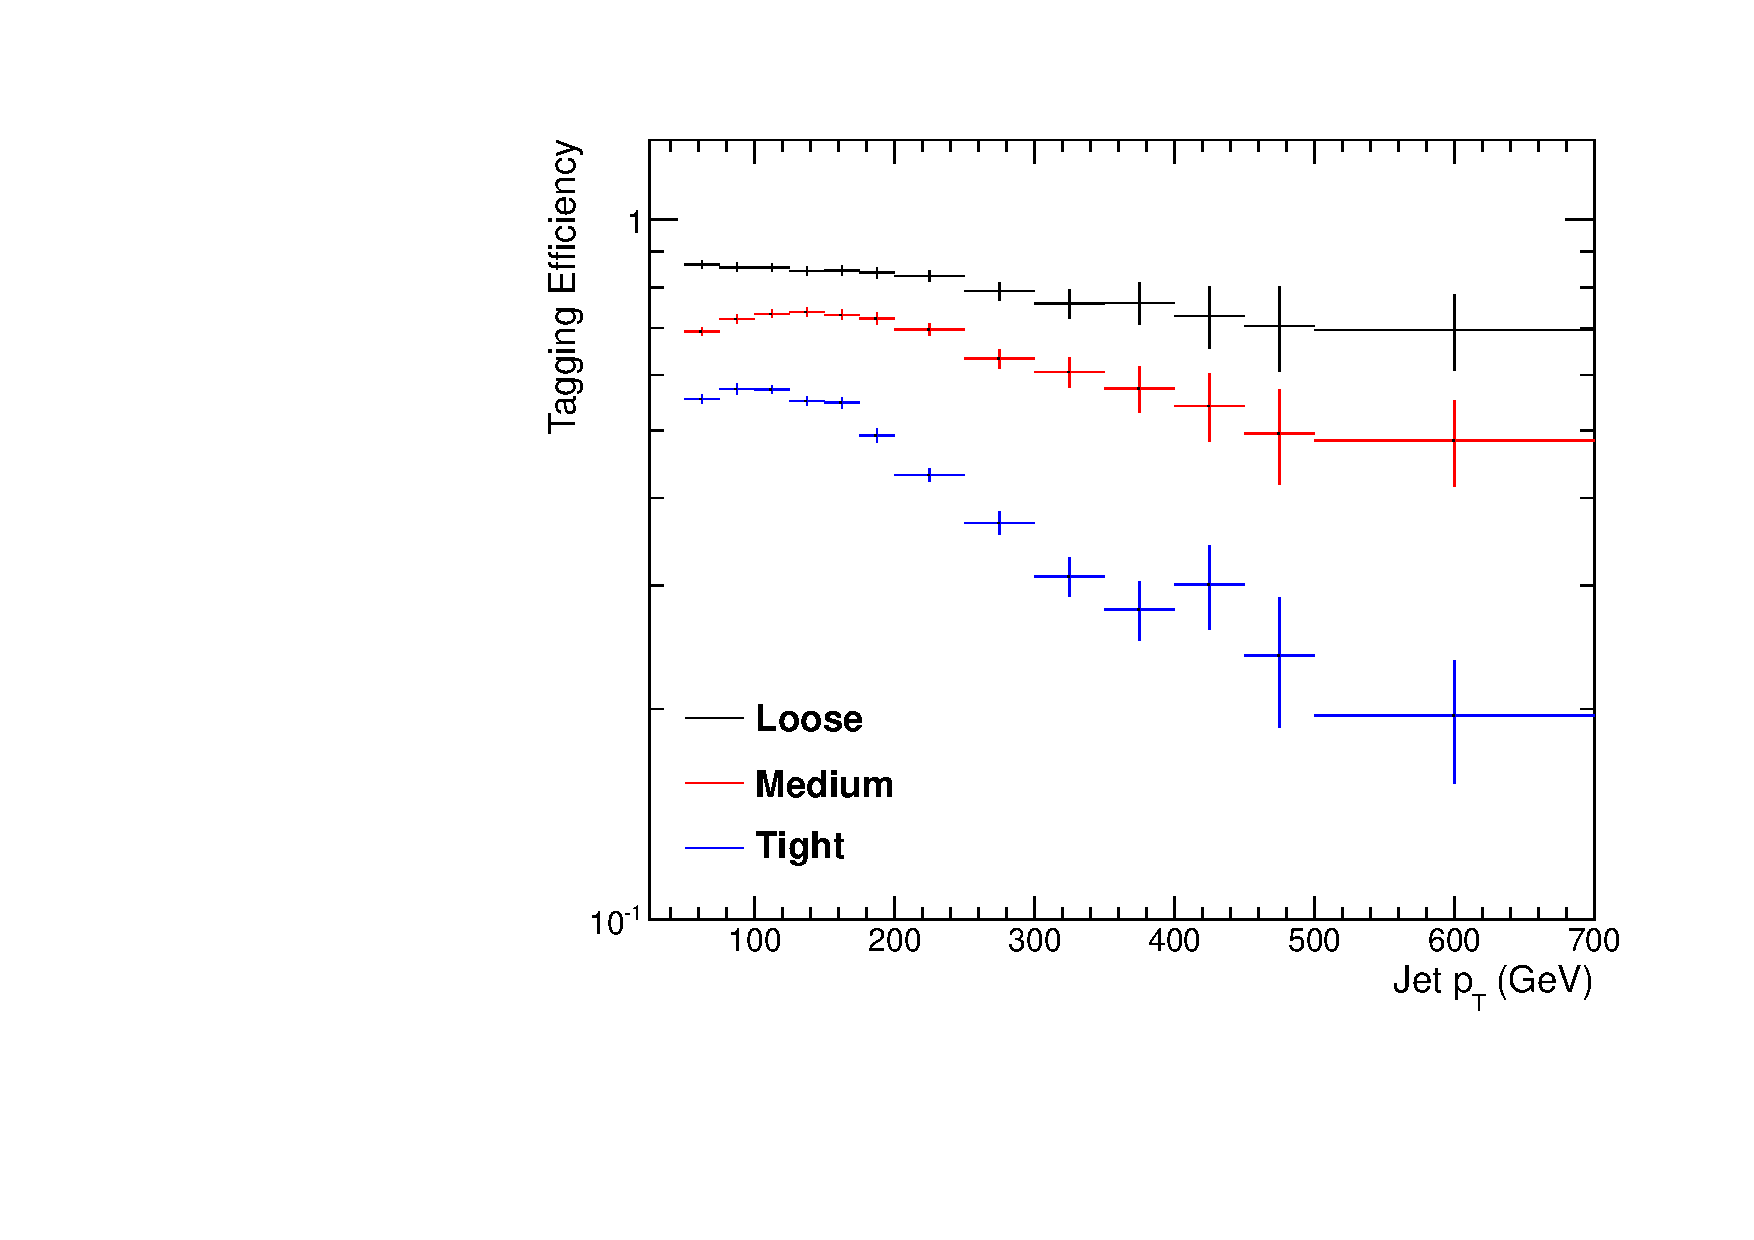
\includegraphics[width = 1.0\linewidth]{plots/bjet_PtDistribution_Htbin_Template_375.pdf}
\centering (a)  b-jets
\end{minipage}
\quad
\begin{minipage}[b]{0.48\linewidth}
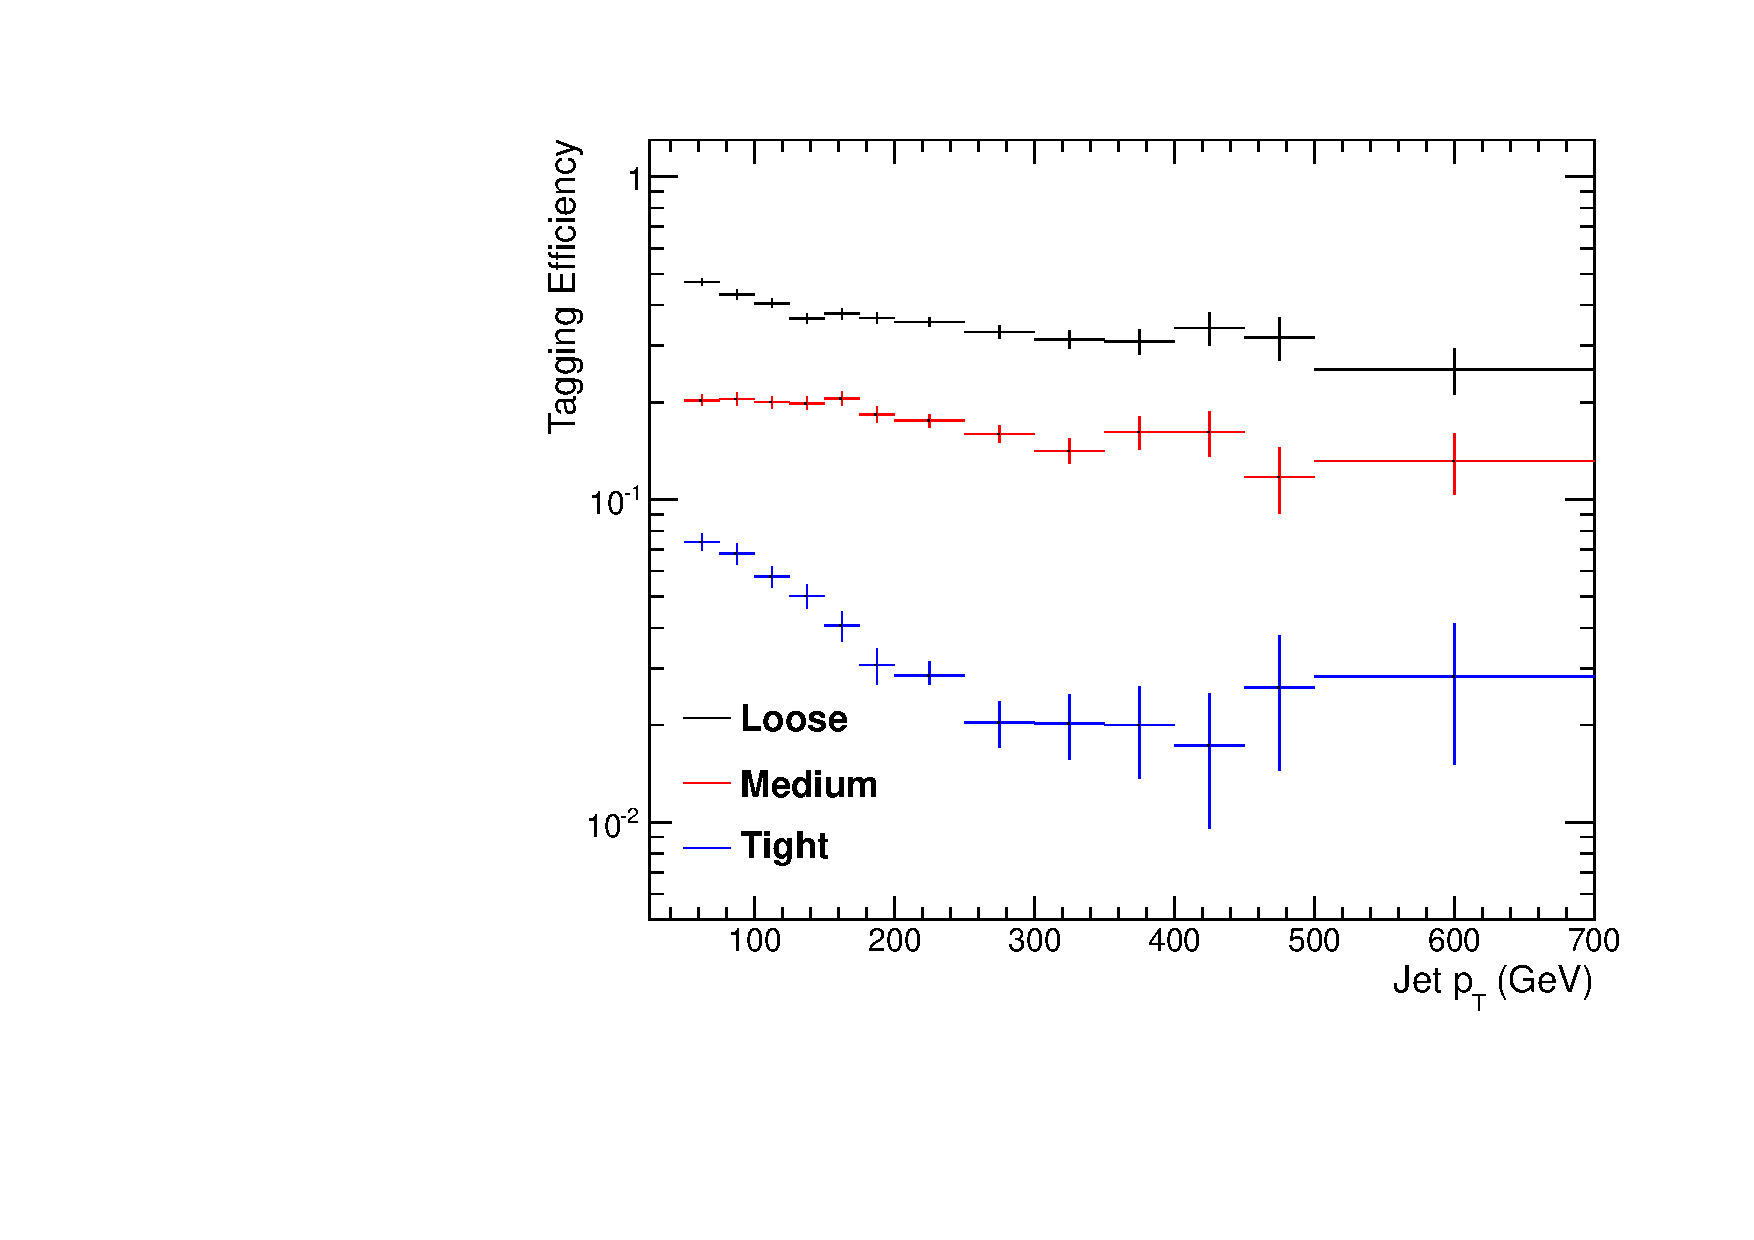
\includegraphics[width = 1.0\linewidth]{plots/cjet_PtDistribution_Htbin_Template_375.pdf}
\centering (b) c-jets
\end{minipage}
\quad
\begin{minipage}[b]{0.48\linewidth}
\centering
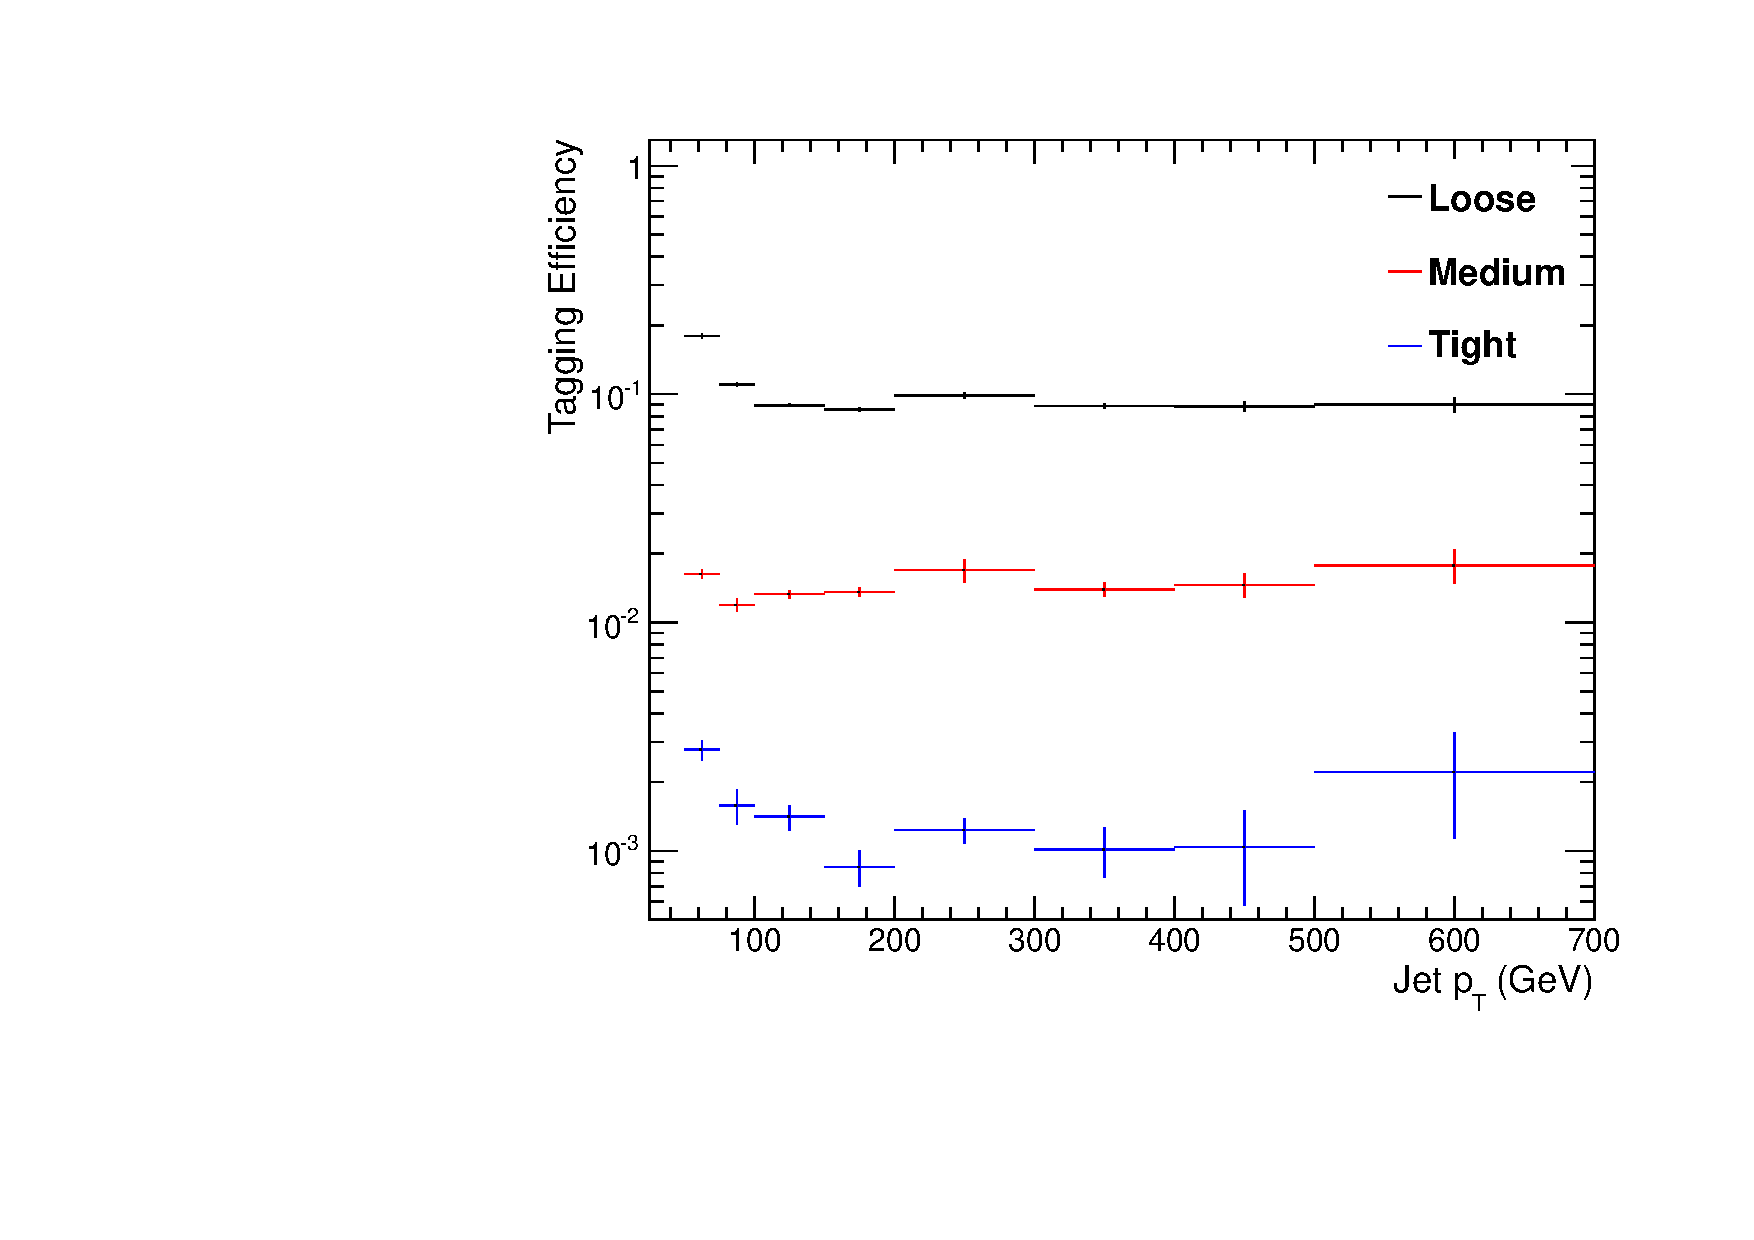
\includegraphics[width = 1.0\linewidth]{plots/lighjet_PtDistribution_Htbin_Template_375.pdf}
\centering (c) light-jets
\end{minipage}
\caption[The b-quark (a), c-quark  (b), and light-quark (c$)$ tagging efficiency as a function of jet \pt, measured in simulation after the application of the \alphat analysis \mupjets control sample selection, in the region \theht $>$ 375.]{The b-quark (a), c-quark  (b), and light-quark (c$)$ tagging efficiency as a function of jet \pt, measured in simulation after the application of \alphat analysis \mupjets control sample selection, in the region \theht $>$ 375. Efficiencies are measured for the three \ac{CSV} working points.}
\label{fig:templatetaggingefficiencies}
\end{figure}
\FloatBarrier

Therefore, before the template shapes are generated via the formula method, the jet \pt and \eta averaged tagging efficiencies of each jet flavour are determined within each individual analysis category. Additionally as already specified in Section (\ref{subsec:formulamethodsf}), the relevant jet \pt and \eta $SF_{b,c,s}$ corrections are then applied to correct the measured b-tagging rate in simulation to that of data. These corrections propagate through to the average determined tagging efficiency for each jet flavour, consequently affecting the final Z0 and Z2 template shape of the \nbreco distribution, determined within each analysis category. 

Using the truth-level flavour information of each of the defined Z0 and Z2 templates and the measured tagging efficiencies of each jet flavour, the template shapes are constructed from simulation via the formula method. These two shapes are then fitted to data in a low $n_{b}^{reco}$ control region (0-2), by allowing the normalisation constants $\theta_{Z0}$ and $\theta_{Z2}$ of the two templates to float. The fits are performed independently within each of the defined analysis category to remove any dependence on the modelling of jet multiplicity between simulation and data. Best fit values of $\theta_{Z0}$ and $\theta_{Z2}$ are used, along with the fixed shape of each template, to extrapolate a \ac{SM} background estimation within the high $n_{b}^{reco}$ signal region (3,4) as shown in Figure \ref{fig:templateexample}. 

 \begin{figure}[!h]
 \centering
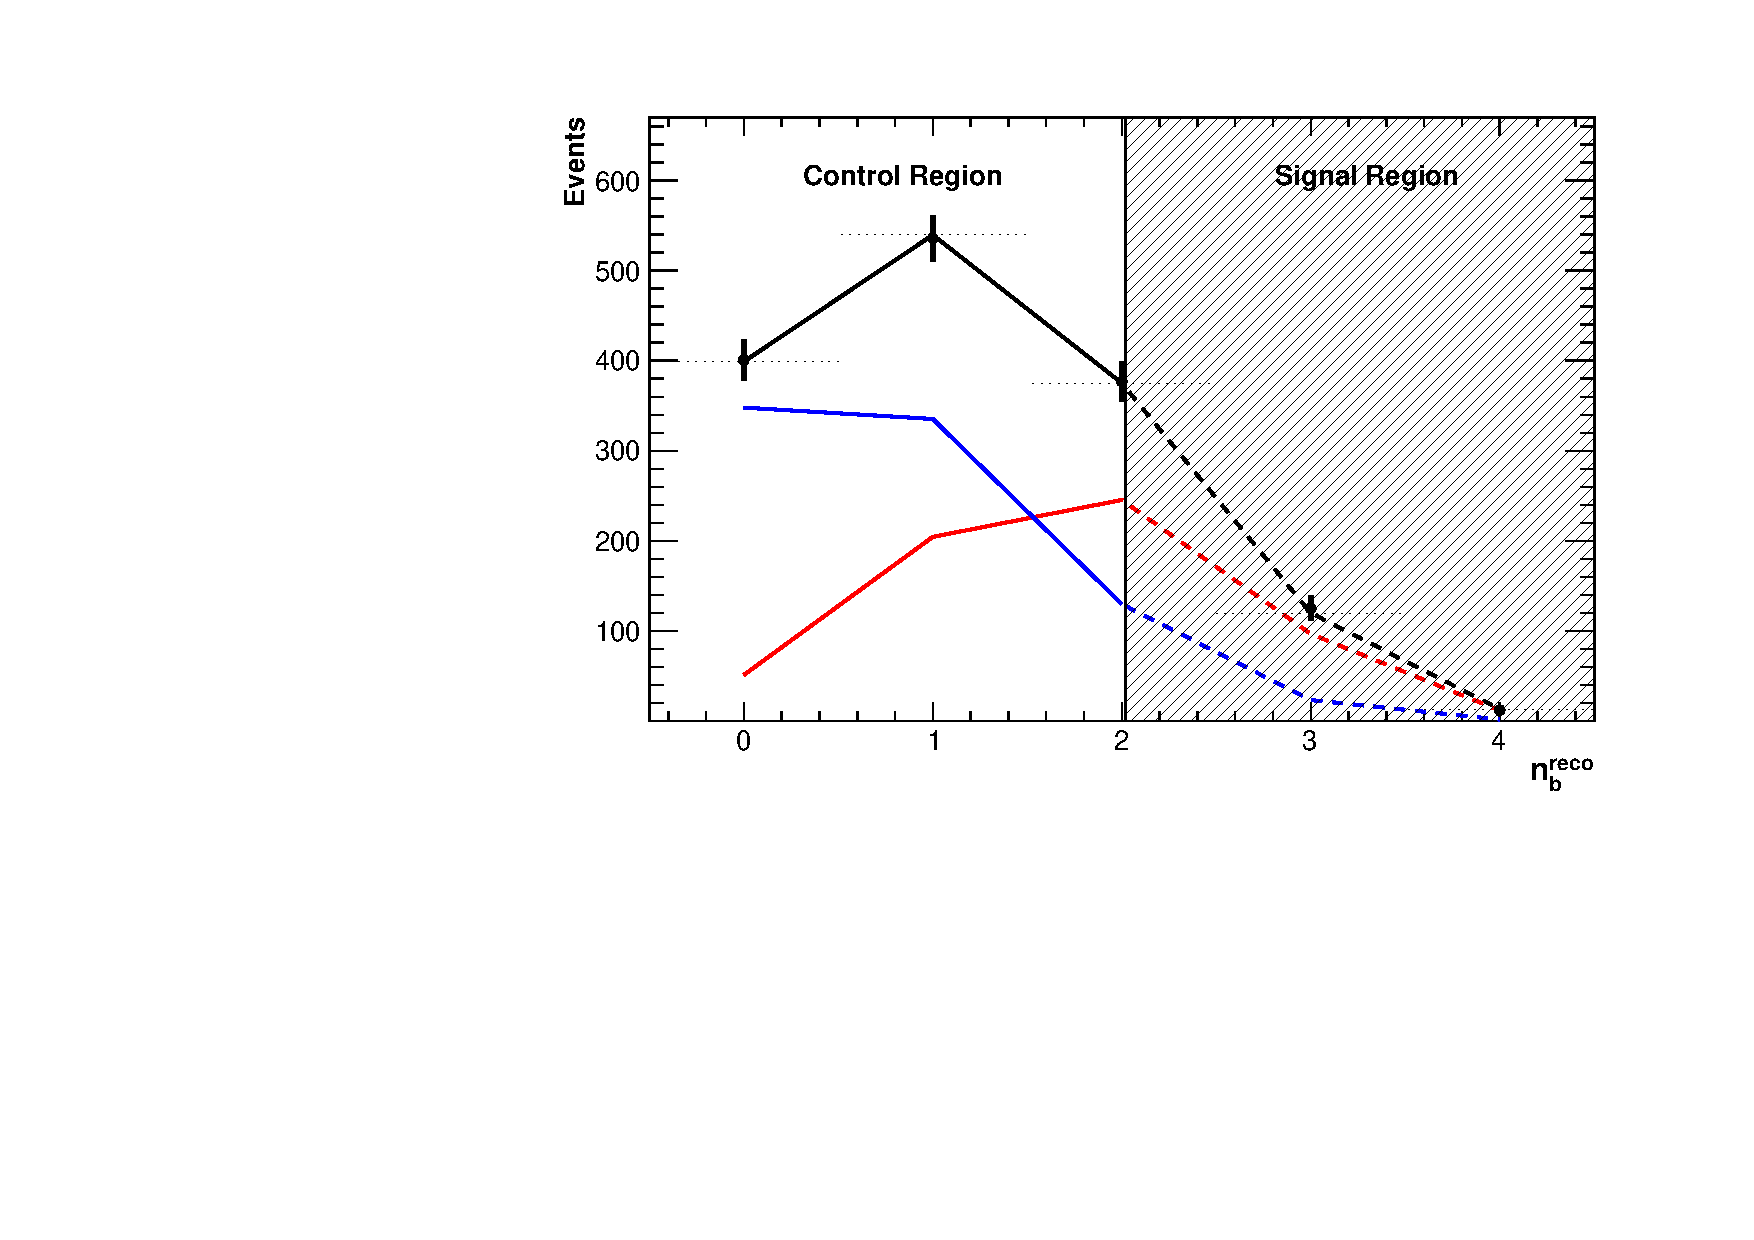
\includegraphics[width=0.60\textwidth]{plots/Template_Example.pdf}
\caption[An example of a template fit with the defined Z0 (blue) and Z2 (red) templates to data within the low \nbreco control region (left).]{An example of a template fit with the defined Z0 (blue) and Z2 (red) templates to data within the low \nbreco control region (left). The shape of the two templates are fixed but the normalisations $\theta_{Z0}$ and $\theta_{Z2}$ are allowed to vary. The best fit values are then applied to extrapolate a combined background prediction from the shaded signal region (right), represented by the dashed black line. Statistical and systemic uncertainties are not shown within this figure.}  
\label{fig:templateexample}
\end{figure}

In deriving the uncertainty on the background prediction the following statistical uncertainties are considered:

\begin{itemize}
\item[]\textbf{Fit uncertainty:} 
 The statistical uncertainty on the normalisation factors $\theta_{Z0}$ and $\theta_{Z2}$ as determined by the fit to data.
\item[]\textbf{Measured tagging efficiency uncertainty:}  
The uncertainty of the template shapes due to the uncertainty on the measured average tagging efficiencies of each jet flavour from simulation. This uncertainty is propagated through to the template prediction for each \nbreco multiplicity by profiling the distribution of the $\theta_{Z0}$ and $\theta_{Z2}$ best-fit values from multiple pseudo-experiments. 

For each pseudo-experiment, a Z0 and Z2 template shape is generated and fitted to data. The tagging efficiencies of each jet flavour used by the formula method to generate the template shape, are determined from a Gaussian distribution centred on the nominal measured efficiency with a width equal to its measured statistical uncertainty. The uncertainties on the nominal $\theta_{Z0}$ and $\theta_{Z2}$ normalisation factors are then determined from the value of the 68th percentile in the best fit $\theta_{Z0}$ and $\theta_{Z2}$ distributions constructed from all of the pseudo-experiments.
\item[]\textbf{Formula method statistical error:}  The statistical uncertainties of the two templates Z0 and Z2 at each \nbreco multiplicity are propagated through to the overall uncertainty. This is due to the finite amount of simulated events used in the formula method to generate the template shapes.
\item[]\textbf{B-tag scale factor systematic error:} When this procedure is applied to data, an additional systematic error is also incorporated into the template uncertainty. This takes into account the uncertainty in correcting the tagging efficiencies measured in simulation to data as first shown in Figures  \ref{fig:btagscalefactors} and \ref{fig:mistagscalefactors}. The systematic uncertainty for each template is determined by varying these simulation to data scale factors ($SF_{\text{b, c, light}}$), up and down by their systematic uncertainties. These scale factor uncertainties are conservatively taken as fully correlated across all jet flavours \cite{btagscalefactor}. The resultant relative difference due to these variations in the template shape at each \nbreco multiplicity of the template, is taken as the systematic uncertainty on the nominal best fit template value.
\end{itemize} 

All statistical and systematic errors are added in quadrature to determine an overall template fit uncertainty at each \nbreco multiplicity in the control and signal regions. These are represented in all figures by a shaded grey band. 

Any large excess in data is an indication that the \nbreco distribution is not adequately described by the \ac{SM} backgrounds encapsulated by the templates. This could mean there are additional \ac{SM} backgrounds that fall within the selection of the analysis that need to be considered, or that there is signal present within the data. This method relies solely on fitting to the shape of the $n_{b}^{reco}$ distribution, and can in principle, be applied to any analysis where the signal hypothesis has a larger underlying b-quark spectra than the \ac{SM} backgrounds. 

However, in the scenario where a \ac{SUSY} signal is present in the search region and contains a low number of underlying b-quarks, the template would be unable to discriminate between this signal and background during the fit in the control region. This will be the case unless the jet \pt distribution of the signal and background were drastically different, in which case there would anyway be many more sensitive and practical ways to establish the presence of a signal in the data than this method. Indeed the template method is only really applicable to the hypothesis that any signal resides at high \nbreco and that the control region 0 $\leq \nbreco \leq 2$ has negligible signal contamination. 

\FloatBarrier
\section{ Application to the \alphat Search}
\label{sec:templateapplication}

As detailed in the previous chapter, the \alphat analysis is a search for supersymmetric particles in all hadronic final states, utilising the kinematic variable \alphat to suppress QCD to a negligible level. \ac{SM} enriched control samples are used to estimate the background within a hadronic signal region. 

The selection for the \mupjets control samples defined in Section (\ref{subsec:controlsampledefinition}) is used to demonstrate the template fitting procedure both conceptually in simulation, and also when applied in data. This is chosen, as such a selection is dominated by events stemming from the \ac{SM} processes with little or no signal contamination from potential new physics due to the selection criteria employed. Contributions from rare \ac{SM} processes with a higher underlying b-quark content (e.g. $t\bar{t}b\bar{b}$) are also found to be negligible from studies in simulation. For these reasons, there is a degree of confidence that the procedure should adequately describe the observations in data when extrapolated to the signal region.

As a departure from the \alphat search strategy described in the previous section, events are categorised according to jet multiplicity categories of 3, 4 and $\geq$ 5 reconstructed jets per event (di-jet events are not included as there is no contribution to the high $n_{b}^{reco}$ signal region (=3, =4)). This is done in order to reduce the kinematic range of the jet \pt's within each category. Furthermore the analysis is split into just three \theht regions, for the purpose of increasing statistics within the control region, 

\begin{itemize}
\item 275-325 \GeV
\item 325-375 \GeV
\item $>$ 375 \GeV
\end{itemize}

contrary to the eight used within the \alphat analysis. Templates for both underlying b-quark content hypotheses are then generated for the nine defined event categories.

\subsection{Proof of Principle in Simulation}
\label{subsec:templateclosuretest}

This template procedure must be first demonstrated to work within simulated events free from any potential signal contamination before it can be applied to data. By combining the relevant ingredients necessary to employ the formula method, \nbreco shape templates are generated individually for each \njet and \theht category using one half of the available simulated events for each \ac{SM} process. In this case, as the template shapes are being fitted to simulation, it is \emph{not} necessary to apply the relevant corrections of the b-tagging rates between data and simulation. 

The other half of simulated events is utilised to provide a statistically independent sample from which the \nbreco distribution is taken directly. The two generated templates are then fit within the low \nbreco (0-2) control region to this pseudo-data, from which a signal region prediction is then extrapolated from the template best fit values. 

The aim of this procedure is to ensure that the template fit can accurately extrapolate the \nbreco distribution within the defined signal region from two independent but kinematically identical samples. Furthermore, as the pseudo-data of the \nbreco distribution is taken directly from simulation, observation of good closure for both the initial fit of the two templates within the control region and after extrapolation to the signal region will serve as a validation of the formula method in recovering the original $n_{b}^{reco}$ distribution itself. 

Results are presented in Figure \ref{fig:template_closure_njet5} for each \ac{CSV} working point in the $\njet \geq 5$ category, using the \mupjets control sample selection and the inclusive \theht$>$ 375 \GeV analysis bin. Additional fit results for other \njet categories which show a similar level of closure can be found within Appendix \ref{app:templatemc}.  The grey bands represent the statistical uncertainty of the template prediction at each \nbreco multiplicity derived from adding in quadrature the statistical uncertainties introduced in the previous section.

\begin{figure}[ht]
\footnotesize
\vspace{5mm}
\centering
\begin{minipage}{.51\textwidth}
\centering
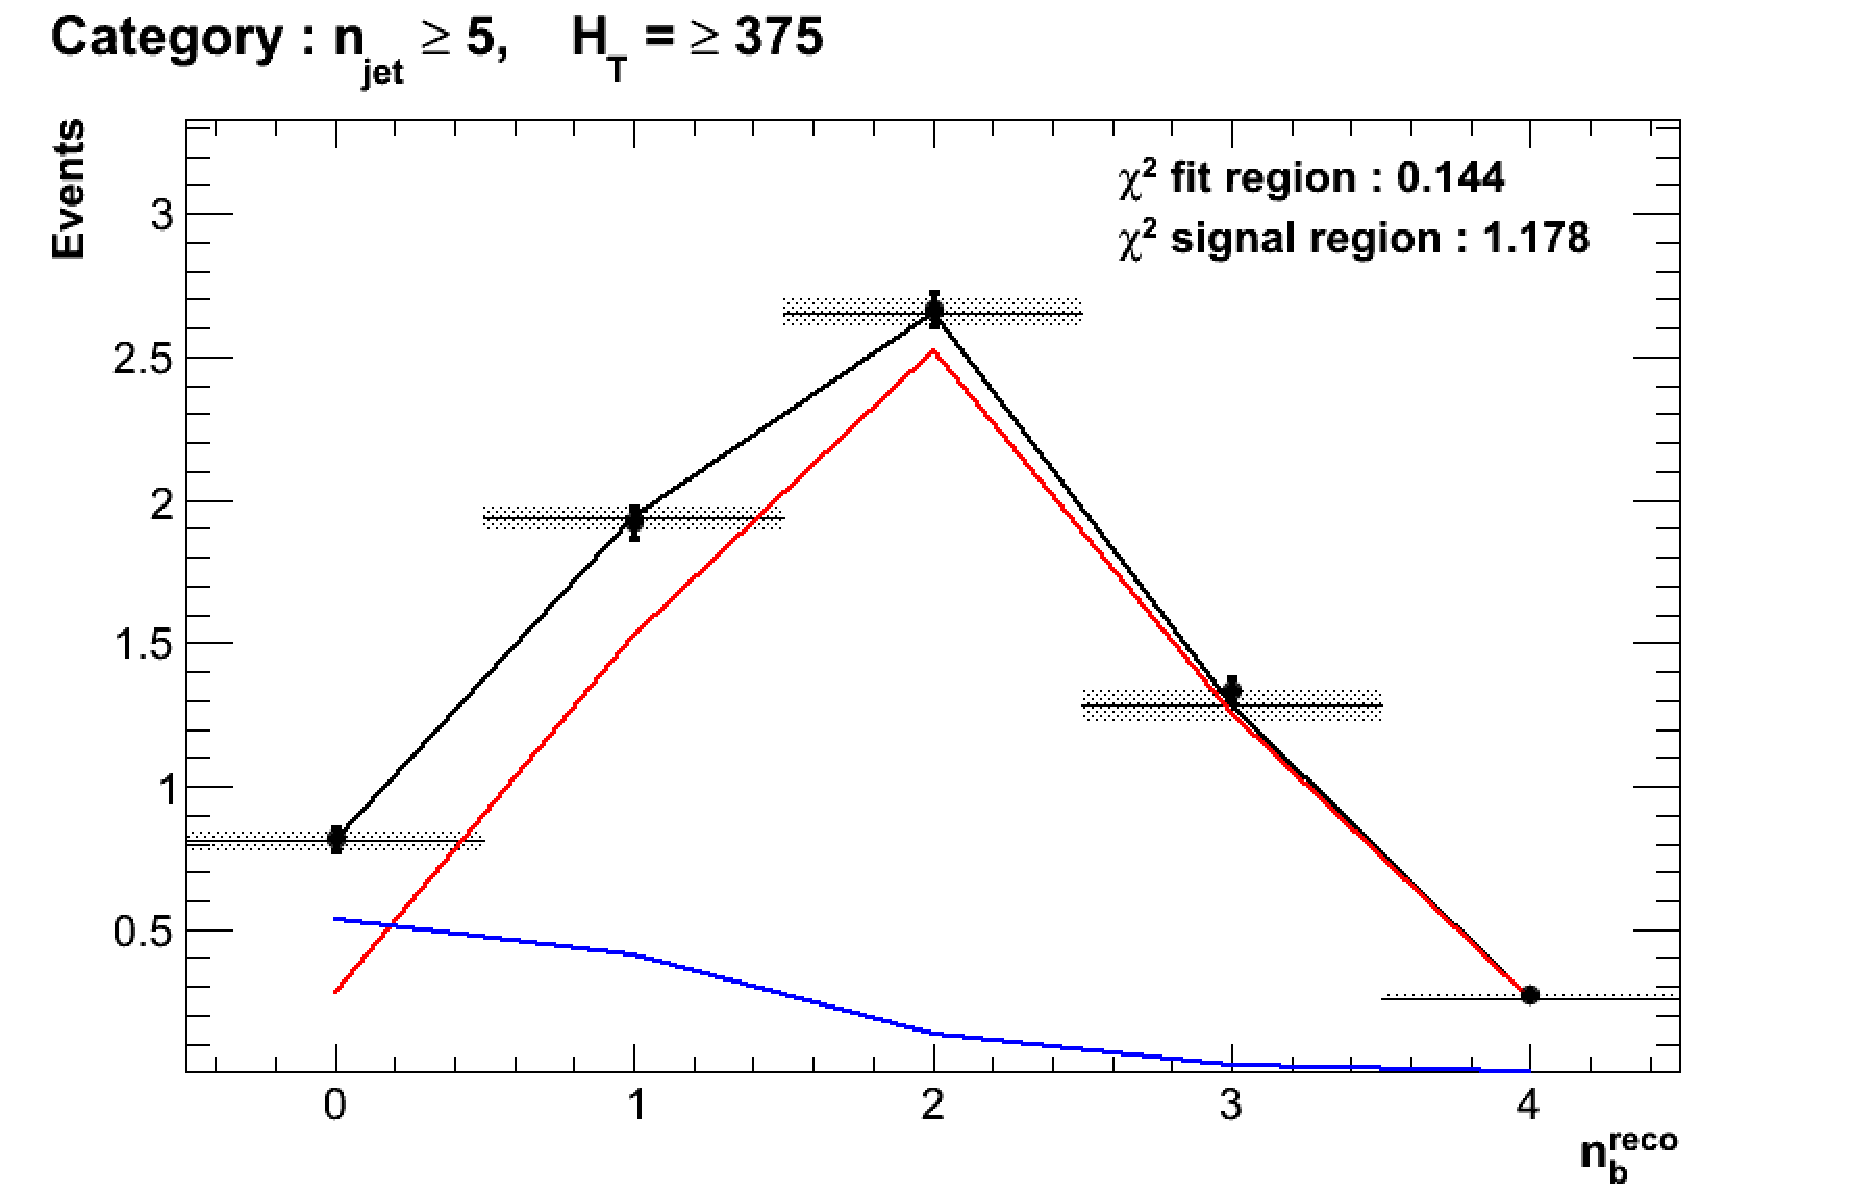
\includegraphics[width = 1.0\linewidth]{plots/ThesisPlots/Final_Fit_To_MC_Normal_Loose_HTBin_OneMuon_Template_375_jet_mult_5.pdf}
\centering (a) Loose working point : $n_{jet} \geq$  5 
\end{minipage}
\quad
\begin{minipage}[b]{0.51\linewidth}
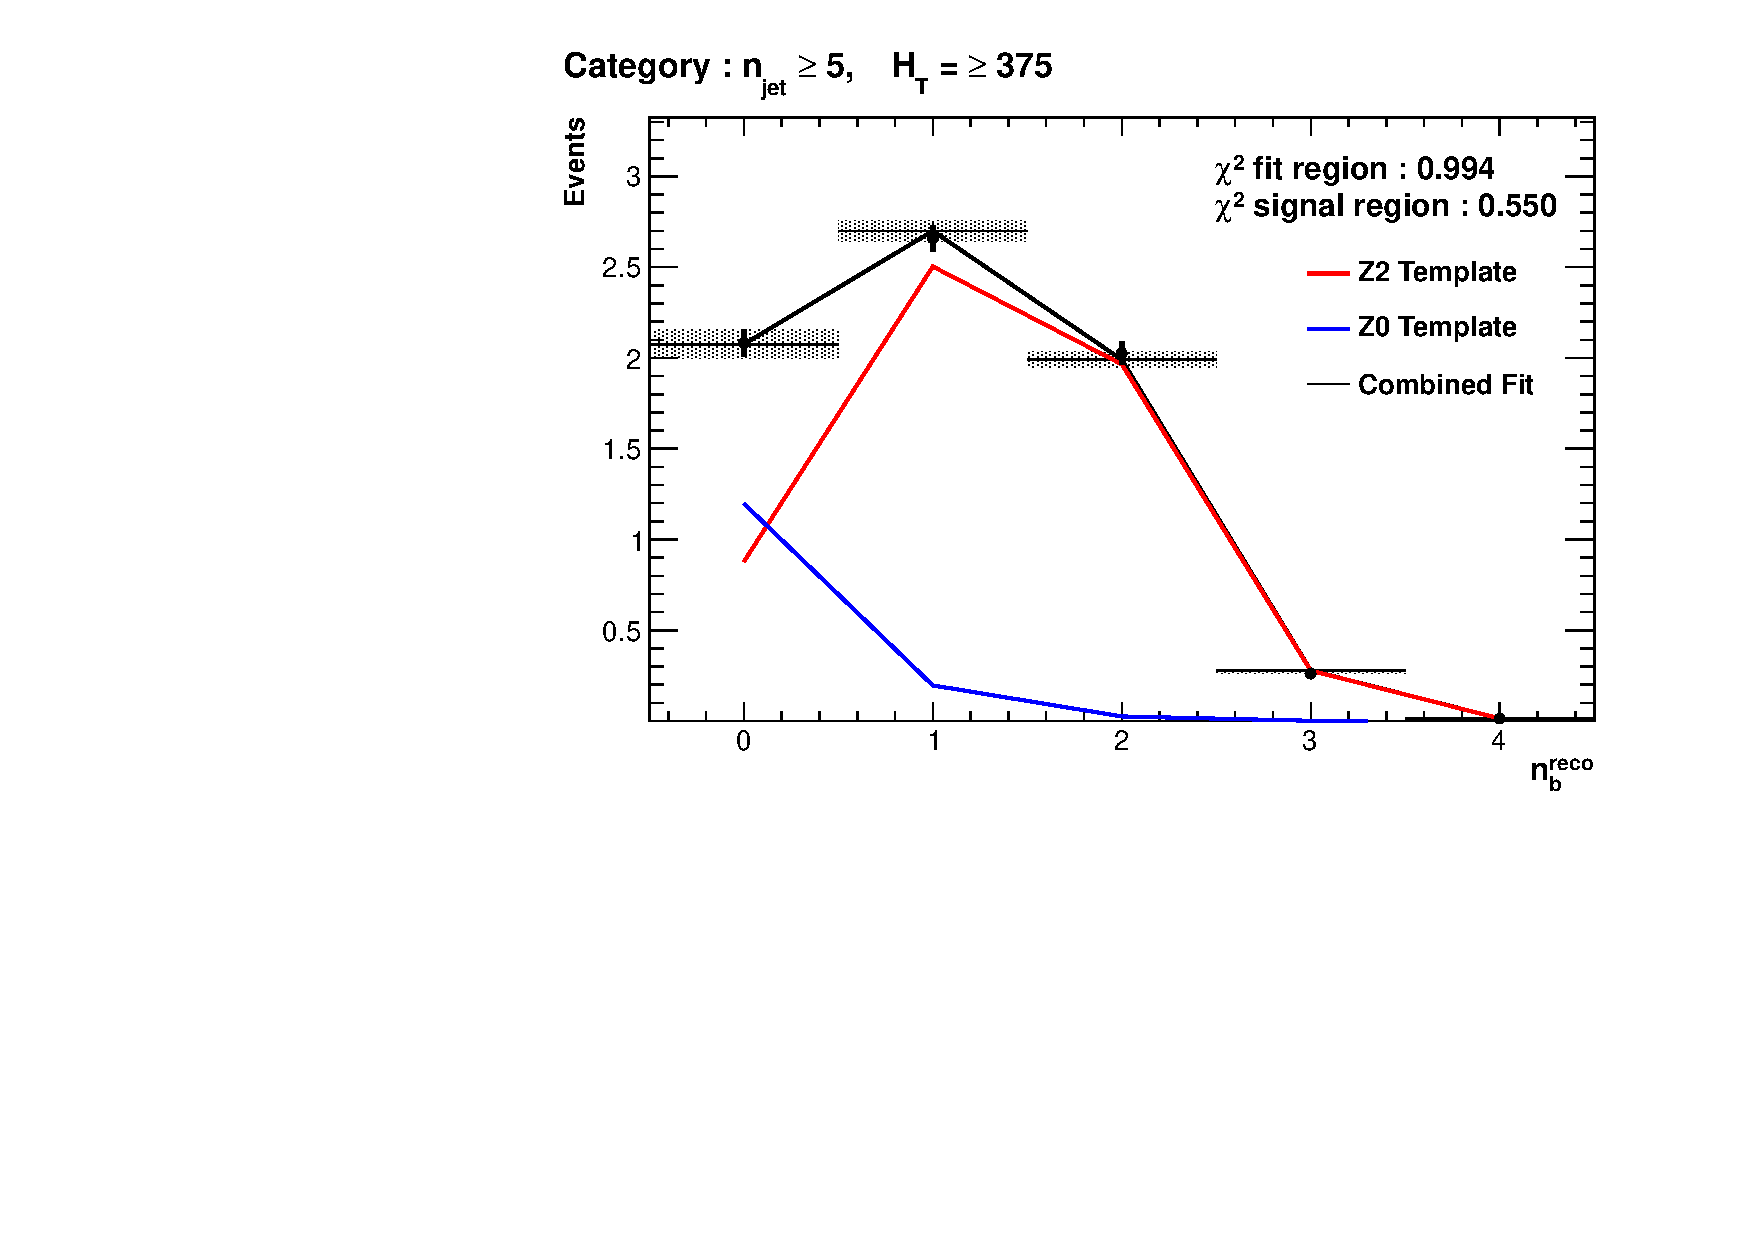
\includegraphics[width = 1.0\linewidth]{plots/ThesisPlots/Final_Fit_To_MC_Normal_Medium_HTBin_OneMuon_Template_375_jet_mult_5.pdf}
\centering (b) Medium working point : $n_{jet} \geq$ = 5 
\end{minipage}
\footnotesize
\centering
\begin{minipage}[b]{0.51\linewidth}
\centering
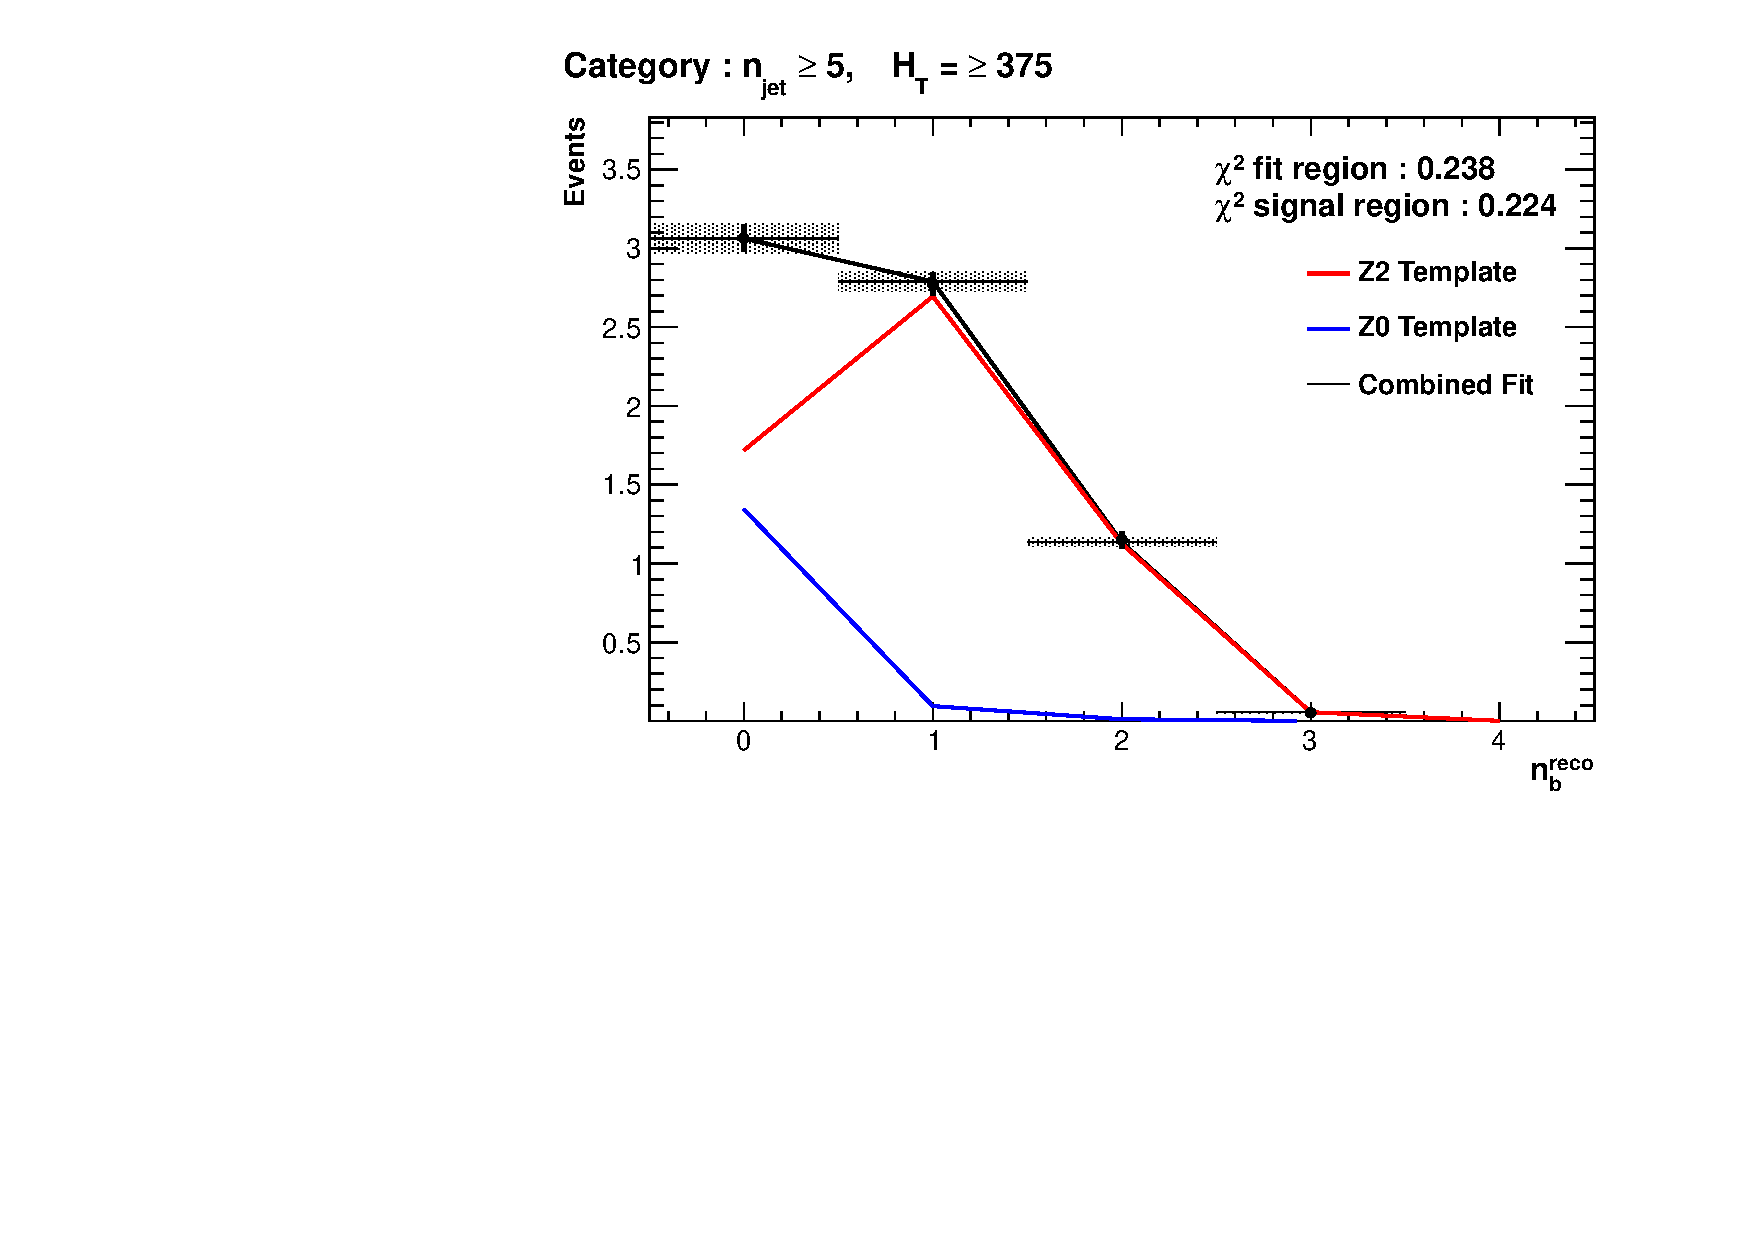
\includegraphics[width = 1.0\linewidth]{plots/ThesisPlots/Final_Fit_To_MC_Normal_Tight_HTBin_OneMuon_Template_375_jet_mult_5.pdf}
\centering (c) Tight working point : $n_{jet} \geq$ 5 
\end{minipage}
\caption[Results of fitting the Z = 0 and Z = 2 templates in the $n_{b}^{reco}$ = 0-2 control region to yields from simulation in the \mupjets control sample for the \theht $>$ 375 \GeV, $n_{jet} \geq 5$ category for all \ac{CSV} working points.]{Results of fitting the Z = 0 and Z = 2 templates in the $n_{b}^{reco}$ = 0-2 control region to yields from simulation in the \mupjets control sample for the \theht $>$ 375 \GeV, $n_{jet} \geq 5$ category  for all \ac{CSV} working points. Data is represented by the black circles with the blue, red and black lines representing the Z=0, Z=2 and combination of both templates respectively. Grey bands represent the uncertainty of the fit. The $\chi^{2}$ parameters represent the goodness of fit to the control and signal region.}
\label{fig:template_closure_njet5}
\end{figure}
\FloatBarrier

The extrapolated fit predictions summed over all \njet multiplicities within the high $n_{b}^{reco}$ signal region, are summarised for all \theht bins and working points in Table \ref{tab:template_mctable}. 

\begin{table}[h!]
\begin{center}
\footnotesize
\begin{tabular*}{0.95\textwidth}{@{\extracolsep{\fill}}llccc}
\cline{1-5}
\multicolumn{2}{c}{\theht} & 275-325 & 325-375 & $>$375 \\

\multicolumn{5}{c}{Loose working point} \\
\hline\hline
Simulation & \multirow{2}{*}{$n_{b} = 3$} & $786.4 \pm 14.7$ & $392.7 \pm 10.3$ & $802.2 \pm 14.4$ \\
Template & & $789.6 \pm 27.5$ & $375.6 \pm 16.6$ & $770.1 \pm 22.9$ \\
Simulation & \multirow{2}{*}{$n_{b} = 4$} & $67.4 \pm 3.9$ & $28.2 \pm 2.7$ & $93.7 \pm 4.9$ \\
Template & & $64.5 \pm 5.9$ & $26.4 \pm 3.3$ & $82.3 \pm 5.8$ \\
\hline
\multicolumn{5}{c}{Medium working point} \\
\hline\hline
Simulation & \multirow{2}{*}{$n_{b} = 3$} & $134.2 \pm 5.8$ & $74.4 \pm 4.5$ & $161.9 \pm 6.3$ \\
Template &  & $129.9 \pm 6.6$ & $68.3 \pm 4.8$ & $159.9 \pm 7.7$ \\
Simulation & \multirow{2}{*}{$n_{b} = 4$} & $1.5 \pm 0.4$ & $0.6 \pm 0.4$ & $3.1 \pm 0.6$ \\
Template & & $1.7 \pm 0.3$ & $0.9 \pm 0.3$ & $3.9 \pm 0.6$ \\
\hline
\multicolumn{5}{c}{Tight working point} \\
\hline\hline
Simulation & \multirow{2}{*}{$n_{b} = 3$} & $28.1 \pm 2.7$ & $13.9 \pm 1.9$ & $29.2 \pm 2.7$ \\
Template & & $25.9 \pm 2.0$ & $12.2 \pm 1.5$ & $28.3 \pm 2.4$ \\
Simulation & \multirow{2}{*}{$n_{b} = 4$} & $0.5 \pm 0.4$ &  -  & $0.2 \pm 0.2$ \\
Template & & $0.1 \pm 0.1$ & $0.1 \pm 0.1$ & $0.2 \pm 0.1$ \\
\end{tabular*}
\end{center}
\caption[Summary of the fit predictions in the $n_{b}^{reco}$ signal region after combination of the $n_{jet} = 3, = 4, \geq 5$ categories compared against yields taken directly from simulation. The predictions are extrapolated from a $n_{b}^{reco}$ = 0, 1, 2 control region and simulation yields are normalised to an integrated luminosity of 10 fb$^{-1}$. ]{Summary of the fit predictions in the $n_{b}^{reco}$ signal region after combination of the $n_{jet} = 3, = 4, \geq 5$ categories compared against yields taken directly from simulation. The fit predictions are extrapolated from a $n_{b}^{reco}$ = 0, 1, 2 control region and simulation yields are normalised to an integrated luminosity of 10 fb$^{-1}$. The uncertainties quoted on the template yields are purely statistical.}\label{tab:template_mctable}
\end{table}

The pull distributions for all the fits performed can be found in Appendix \ref{app:templatepulldistributions}, and are compatible with a mean of zero and standard deviation of one, showing no obvious bias to the fitting procedure. Each of the fits performed show good compatibility between the template shapes and data from simulation within the defined control region, with additional good overall agreement also observed for extrapolation to the signal region as shown in Table \ref{tab:template_mctable}. This validates both the formula method used in the generation of the template shapes as well as the method of predicting the \ac{SM} background in the high \nbreco signal region. 

The application of this method to the same selection in a data control sample is now used to demonstrate necessary control over the efficiency and mis-tagging rates when b-tagging scale factors are applied, and to test the assumption of no signal contamination with the \mupjets control sample.

\subsection{Results in a Data Control Sample}
\label{subsec:templatedataresults}

The procedure is now applied to the 2012 8 \TeV dataset in the \mupjets control sample, to establish the validity of this method in data. The relevant data to simulation b-tagging scale factors are applied to produce corrected values of the efficiency and mis-tagging rates within each analysis category \cite{btagscalefactor}. 

Figure \ref{fig:template_data_med_njet5} shows the results of the templates derived from simulation to each of the three defined \theht bins, in the $n_{jet} \geq 5$ category for the medium working point \ac{CSV} tagger (the same working point used within the \alphat analysis).  Grey bands represent the previously detailed statistical uncertainty of the fit combined in quadrature with the systematic uncertainties of varying up and down the simulation to data scale factors by their b-tag scale factor systematic uncertainties. Additional fit results for other jet multiplicities are found in Appendix \ref{app:templatedata}.
 
 \begin{figure}[ht]
\footnotesize
\centering
\begin{minipage}[b]{0.50\linewidth}
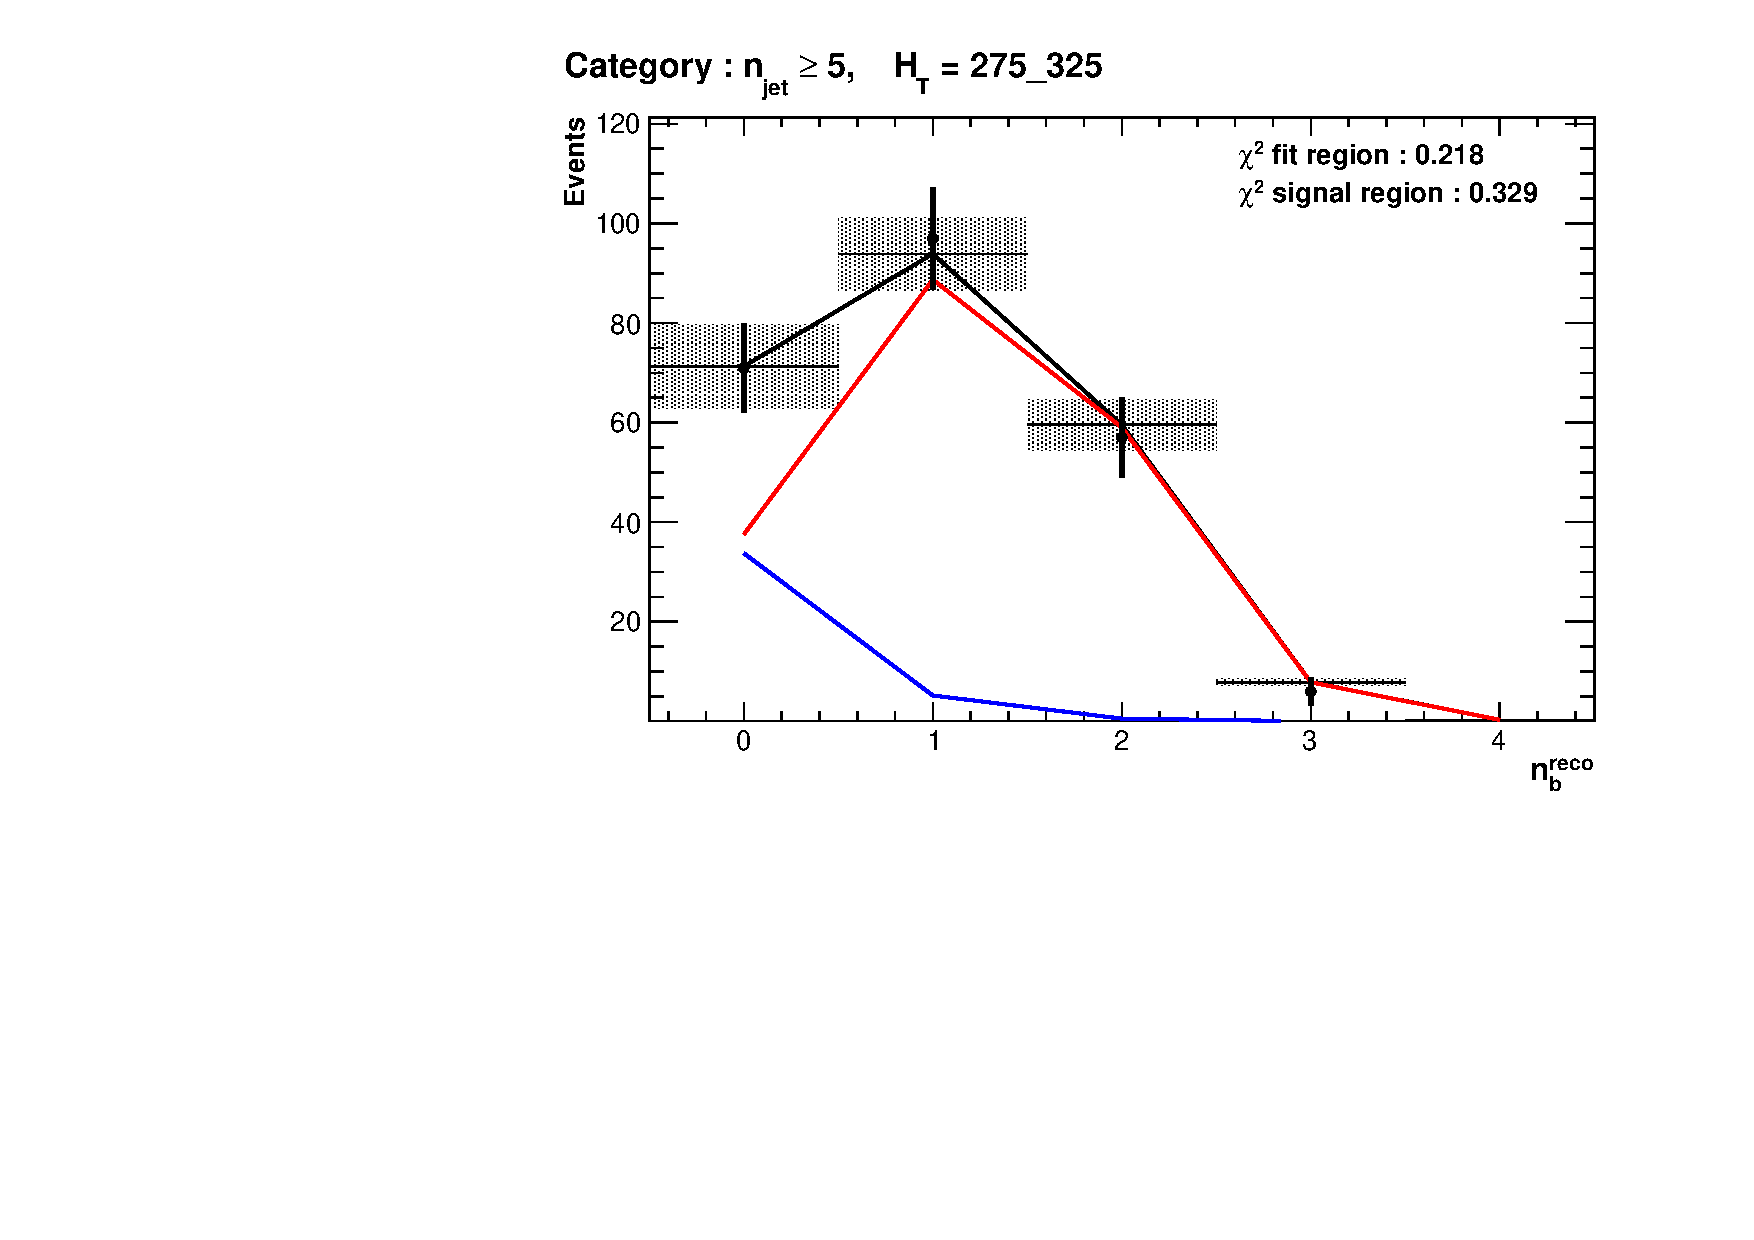
\includegraphics[width = 1.0\linewidth]{plots/ThesisPlots/Final_Fit_To_Data_Normal_Medium_HTBin_OneMuon_275_325_jet_mult_5.pdf}
\centering (a) $n_{jet} \geq$  5 , 275 $<$ \theht $<$ 325
\end{minipage}
\footnotesize
\centering
\begin{minipage}[b]{0.50\linewidth}
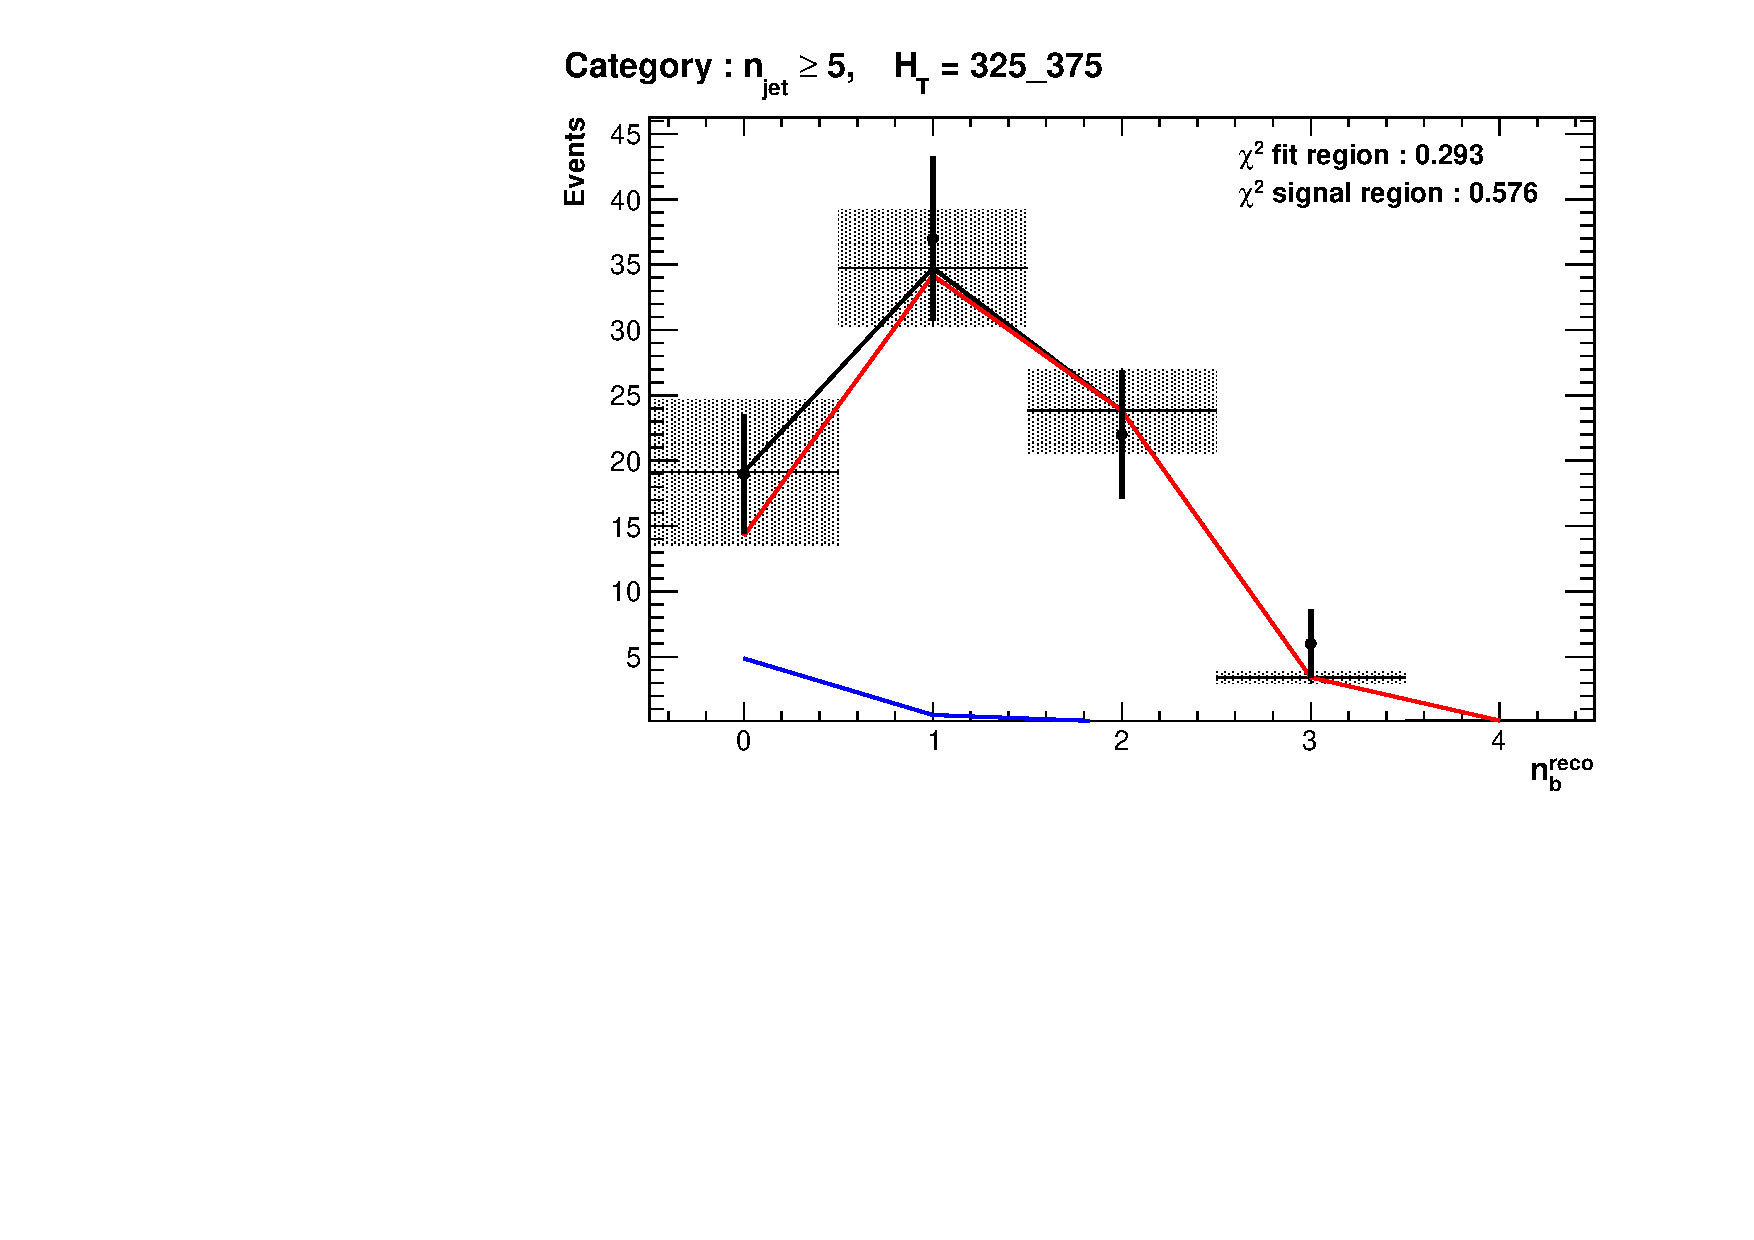
\includegraphics[width = 1.0\linewidth]{plots/ThesisPlots/Final_Fit_To_Data_Normal_Medium_HTBin_OneMuon_325_375_jet_mult_5.pdf}
\centering (b) $n_{jet} \geq$ = 5 , 325 $<$ \theht $<$ 375 
\end{minipage}
\footnotesize
\centering
\begin{minipage}[b]{0.51\linewidth}
\centering
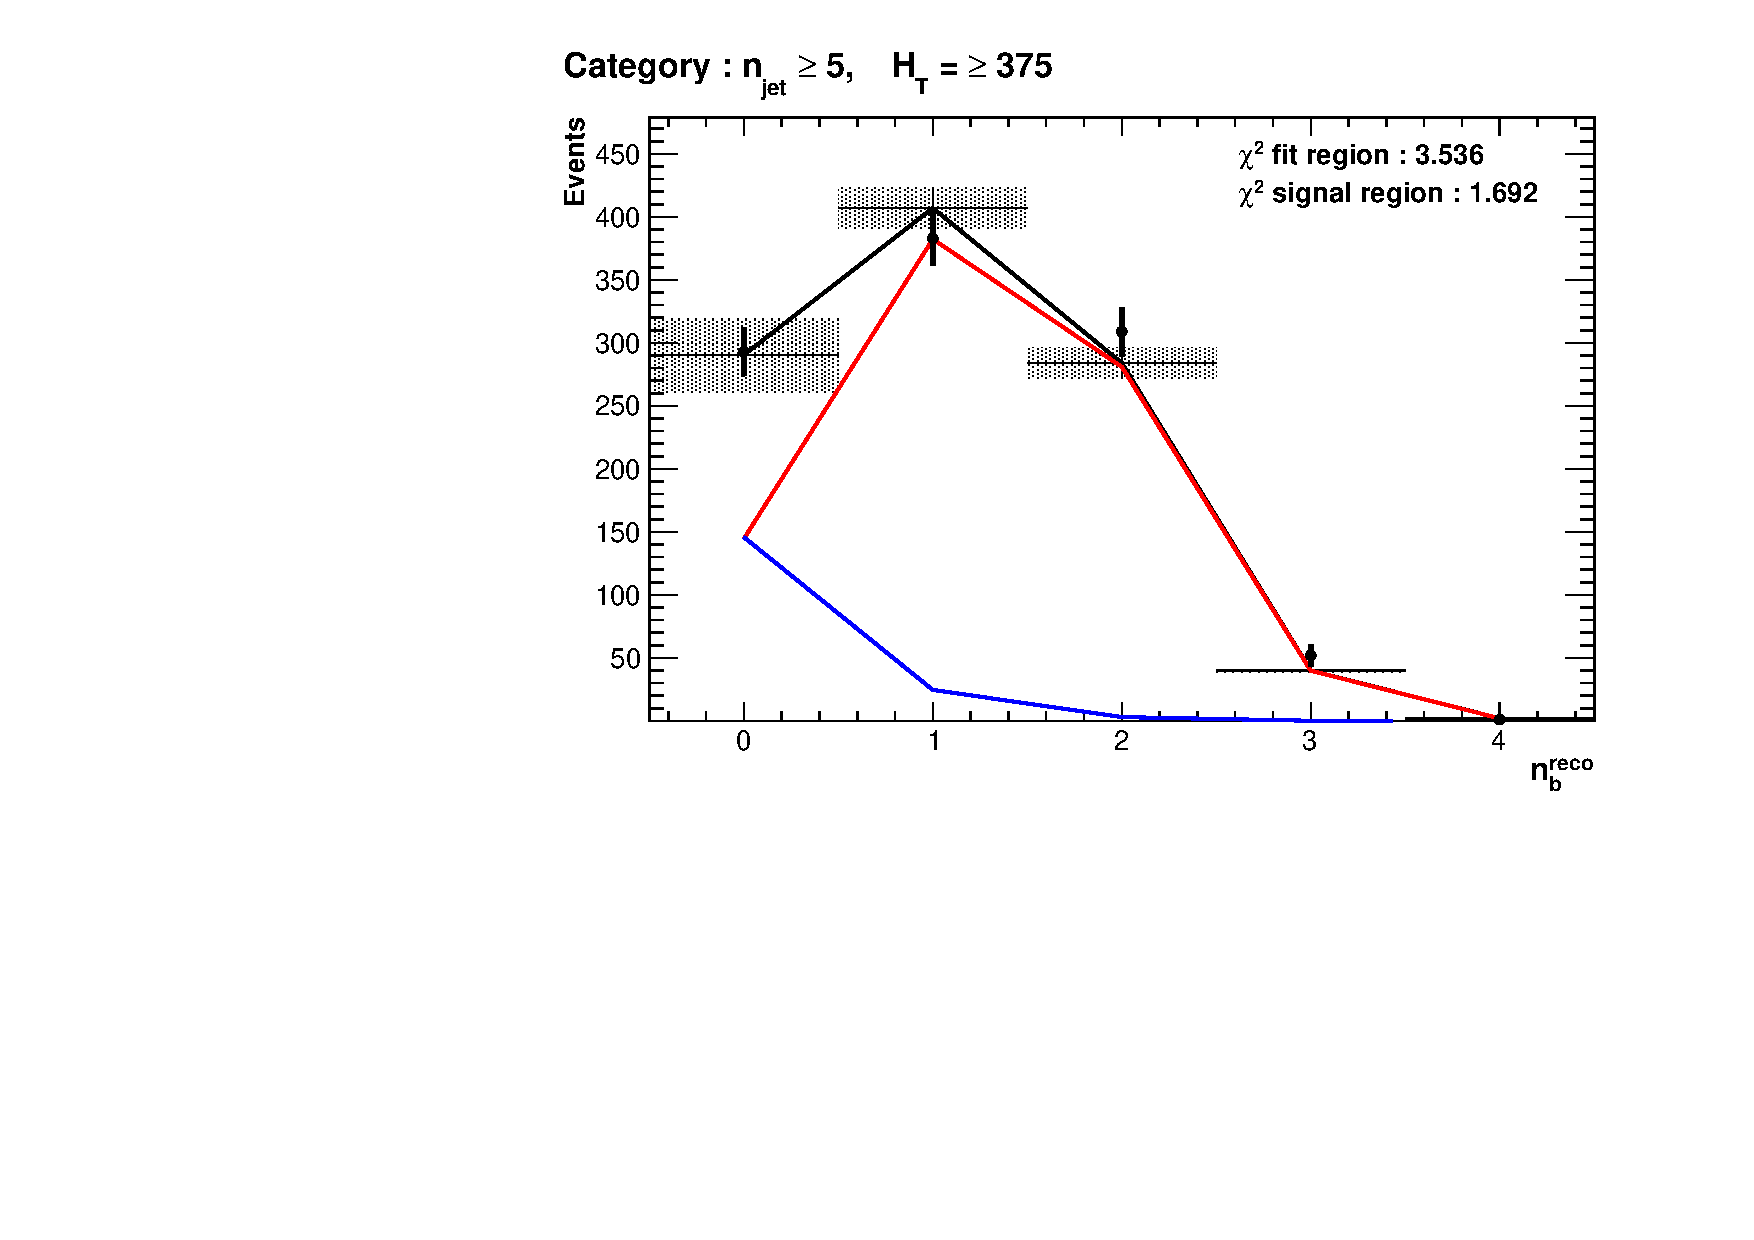
\includegraphics[width = 1.0\linewidth]{plots/ThesisPlots/Final_Fit_To_Data_Normal_Medium_HTBin_OneMuon_Template_375_jet_mult_5.pdf}
\centering (c) $n_{jet} \geq$ 5 , \theht $>$ 375 
\end{minipage}
\caption[Results of fitting the Z = 0 and Z = 2 templates in the $n_{b}^{reco}$ = 0-2 control region to data from the \mupjets control sample, for the \ac{CSV} medium working point, with $n_{jet} \geq 5$ in each \theht category.]{Results of fitting the Z = 0 and Z = 2 templates in the $n_{b}^{reco}$ = 0-2 control region to data from the \mupjets control sample, for the \ac{CSV} medium working point, with $n_{jet} \geq 5$ in each \theht category. Data is represented by the black circles with the blue, red and black lines representing the Z=0, Z=2 and combination of both templates respectively. Grey bands represent the uncertainty of the fit. The $\chi^{2}$ parameters represent the goodness of fit to the control and signal region.}
\label{fig:template_data_med_njet5}
\end{figure}

The numerical results and extrapolation to the $n_{b}^{reco} =$3, =4 bins for all \theht and working points, is shown in Table \ref{tab:template_datatable}.

\begin{table}[h!]
\begin{center}
\footnotesize
\begin{tabular*}{0.95\textwidth}{@{\extracolsep{\fill}}lllll}
\cline{1-5}
\multicolumn{2}{c}{\theht} & 275-325 & 325-375 & $>$375 \\
\multicolumn{5}{c}{Loose working point} \\
\hline\hline
Data & \multirow{2}{*}{$n_{b} = 3$} & 838 & 394 & 717\\
Template & & $871.8 \pm 46.9$ & $369.9 \pm 23.7$ & $678.5 \pm 42.5$ \\
Data & \multirow{2}{*}{$n_{b} = 4$} & 81 & 43 & 81 \\
Template & & $79.4 \pm 9.9$ & $32.9 \pm 4.2$ & $74.4 \pm 10.0$ \\
\hline
\multicolumn{5}{c}{Medium working point} \\
\hline\hline
Data & \multirow{2}{*}{$n_{b} = 3$} & 137 & 79 & 152 \\
Template & & $132.6 \pm 9.3$ & $69.8 \pm 5.4$ & $133.1 \pm 10.8$ \\
Data & \multirow{2}{*}{$n_{b} = 4$} & 1 & 1 & 3 \\
Template & & $1.9 \pm 0.4$ & $0.9 \pm 0.3$ & $3.2 \pm 0.6$ \\
\hline
\multicolumn{5}{c}{Tight working point} \\
\hline\hline
Data & \multirow{2}{*}{$n_{b} = 3$} & 24 & 15 & 25 \\
Template & & $22.3 \pm 1.9$ & $12.1 \pm 1.2$ & $20.3 \pm 2.4$ \\
Data & \multirow{2}{*}{$n_{b} = 4$} & 0 & 0 & 1 \\
Template & & $0.1 \pm 0.1$ & $0.1 \pm 0.1$ & $0.2 \pm 0.1$ \\
\end{tabular*}
\end{center}
\caption[Summary of the fit predictions in the $n_{b}^{reco}$ signal region of the \mupjets control sample, after combination of the $n_{jet} = 3, = 4, \geq 5$ categories.. The predictions are extrapolated from a $n_{b}^{reco}$ = 0, 1, 2 control region using 11.4 fb$^{-1}$ of $\sqrt{s} = 8$\TeV data.]{Summary of the fit predictions in the $n_{b}^{reco}$ signal region of the \mupjets control sample, after combination of the $n_{jet} = 3, = 4, \geq 5$ categories. The predictions are extrapolated from a $n_{b}^{reco}$ = 0, 1, 2 control region using 11.4 fb$^{-1}$ of $\sqrt{s} = 8$\TeV data. The uncertainties quoted on the template yields are a combination of statistical and systematic uncertainties.}\label{tab:template_datatable}
\end{table}

When this method is applied to the \mupjets control sample, it is expected that good agreement would be observed between the template predictions and observation in the absence of signal contamination. The good compatibility for all working points as shown in the table, demonstrate that this is the case and that the method is able to accurately predict the background yields. However the assumption of negligible signal contamination can no longer made when applied to the hadronic signal region of the \alphat search, where agreement between estimated backgrounds and observations in data is now not necessarily expected. Therefore a departure between the extrapolated background estimation and observation in data could point to a potential supersymmetric signature containing a larger number of b-quarks in its final state.
 
\subsection{Application to the \alphat Hadronic Search Region}
\label{subsec:templatedataresults}

As an accompaniment to the background estimation methods outlined in the \alphat search, the b-tag template method offers a complementary way of testing the \ac{SM} only background hypothesis within the hadronic signal region of the search. In the presence of a natural \ac{SUSY} signature mediated by a light gluino and containing four underlying $\widetilde{b}$ or $\widetilde{t}$ squarks, which subsequently decay to t or b-quarks, the number of reconstructed \nbreco = 3, $= 4$ events will be enhanced.

Figure \ref{fig:template_data_signal_njet5} shows the  the results of the template shapes derived from simulation and fitted to data for each of the three \ac{CSV} working points, in the $n_{jet} \geq 5$, \theht $>$ 375 \GeV category.  Grey bands represent the statistical uncertainty of the fit combined in quadrature with the systematic uncertainties of varying the simulation to data scale factors up and down by their measured systematic uncertainties.  Additional fit results for other jet multiplicities are found in Appendix \ref{app:templatedata_signal}.

\vspace*{100px}

\begin{figure}[ht]
\footnotesize
\centering
\begin{minipage}[b]{0.51\linewidth}
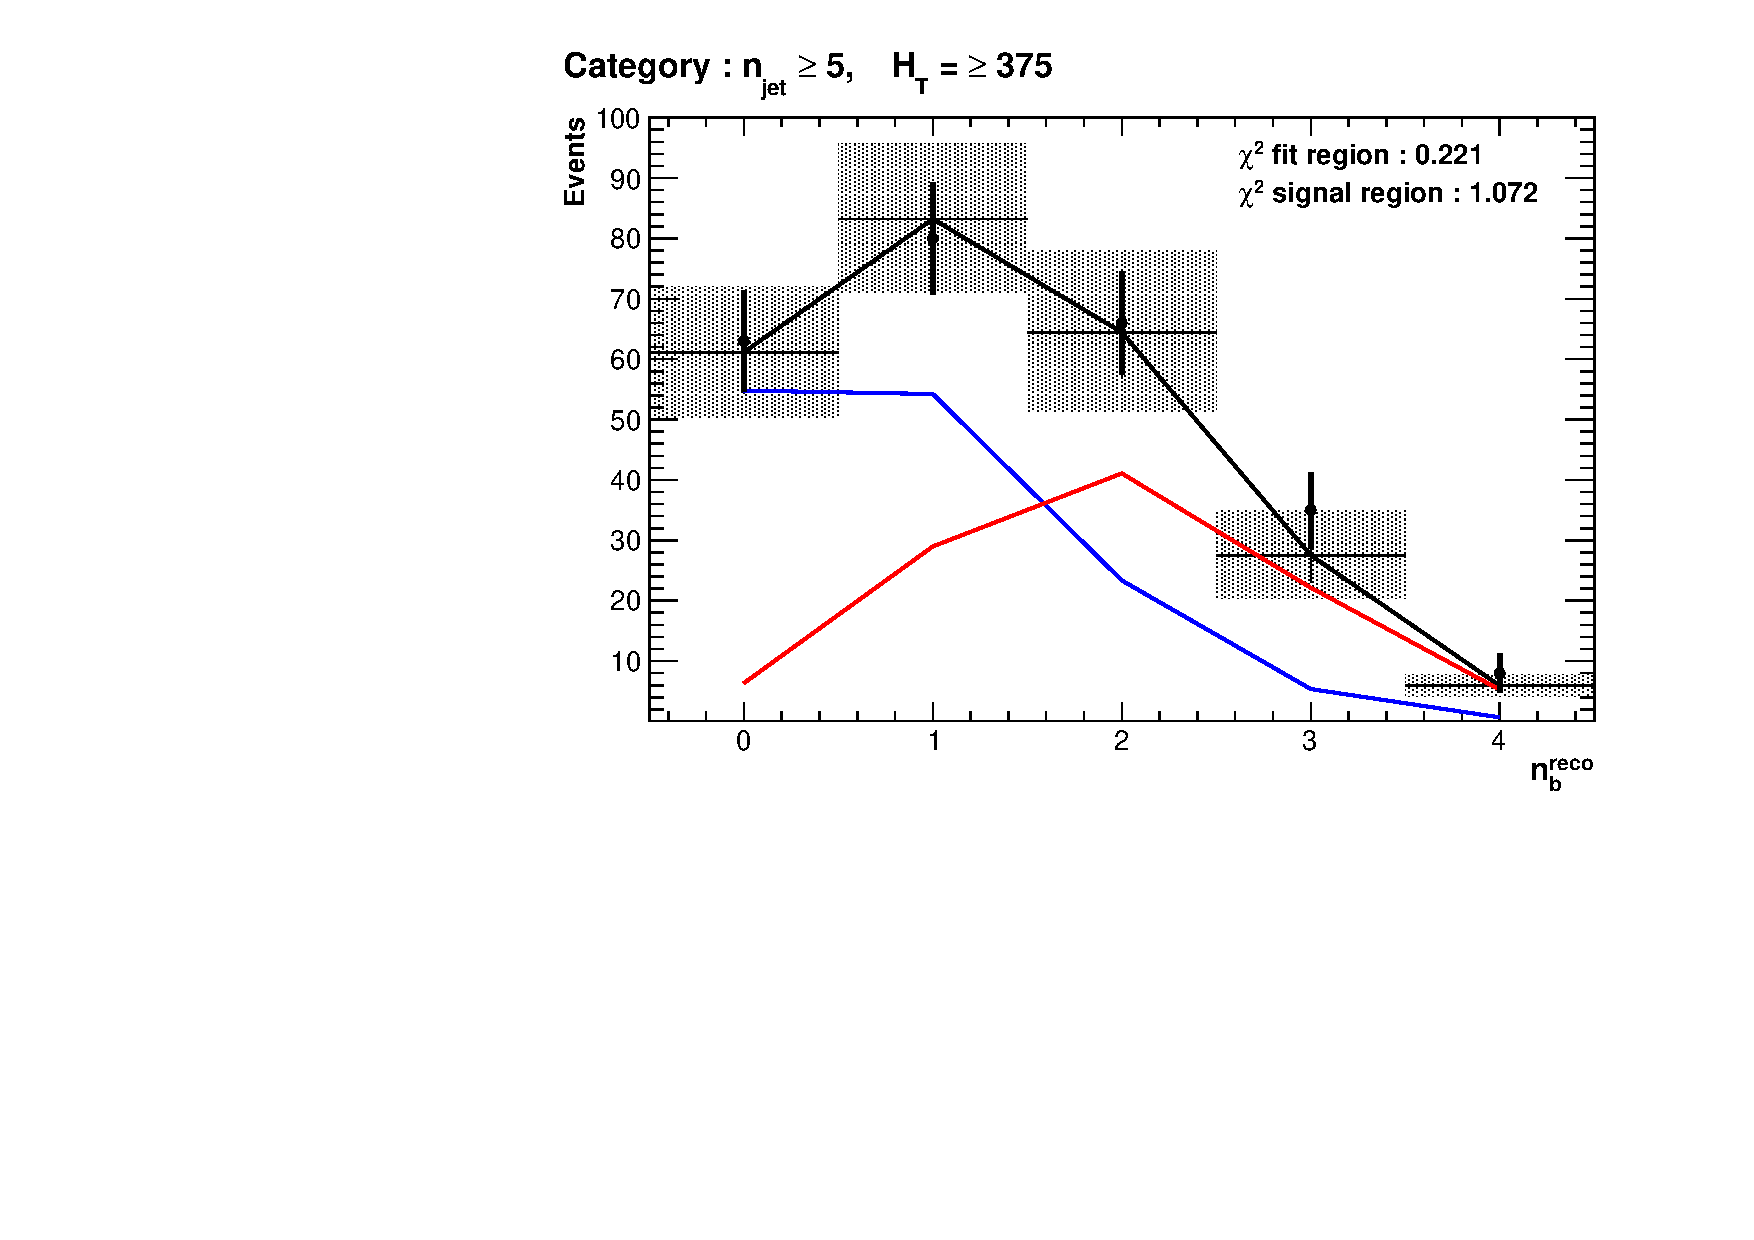
\includegraphics[width = 1.0\linewidth]{plots/TemplatesSignal/Final_Fit_To_Data_Normal_Loose_HTBin_Template_375_jet_mult_5.pdf}
\centering (a) Loose working point : $n_{jet} \geq$  5 , \theht $>$ 375
\end{minipage}
\footnotesize
\begin{minipage}[b]{0.51\linewidth}
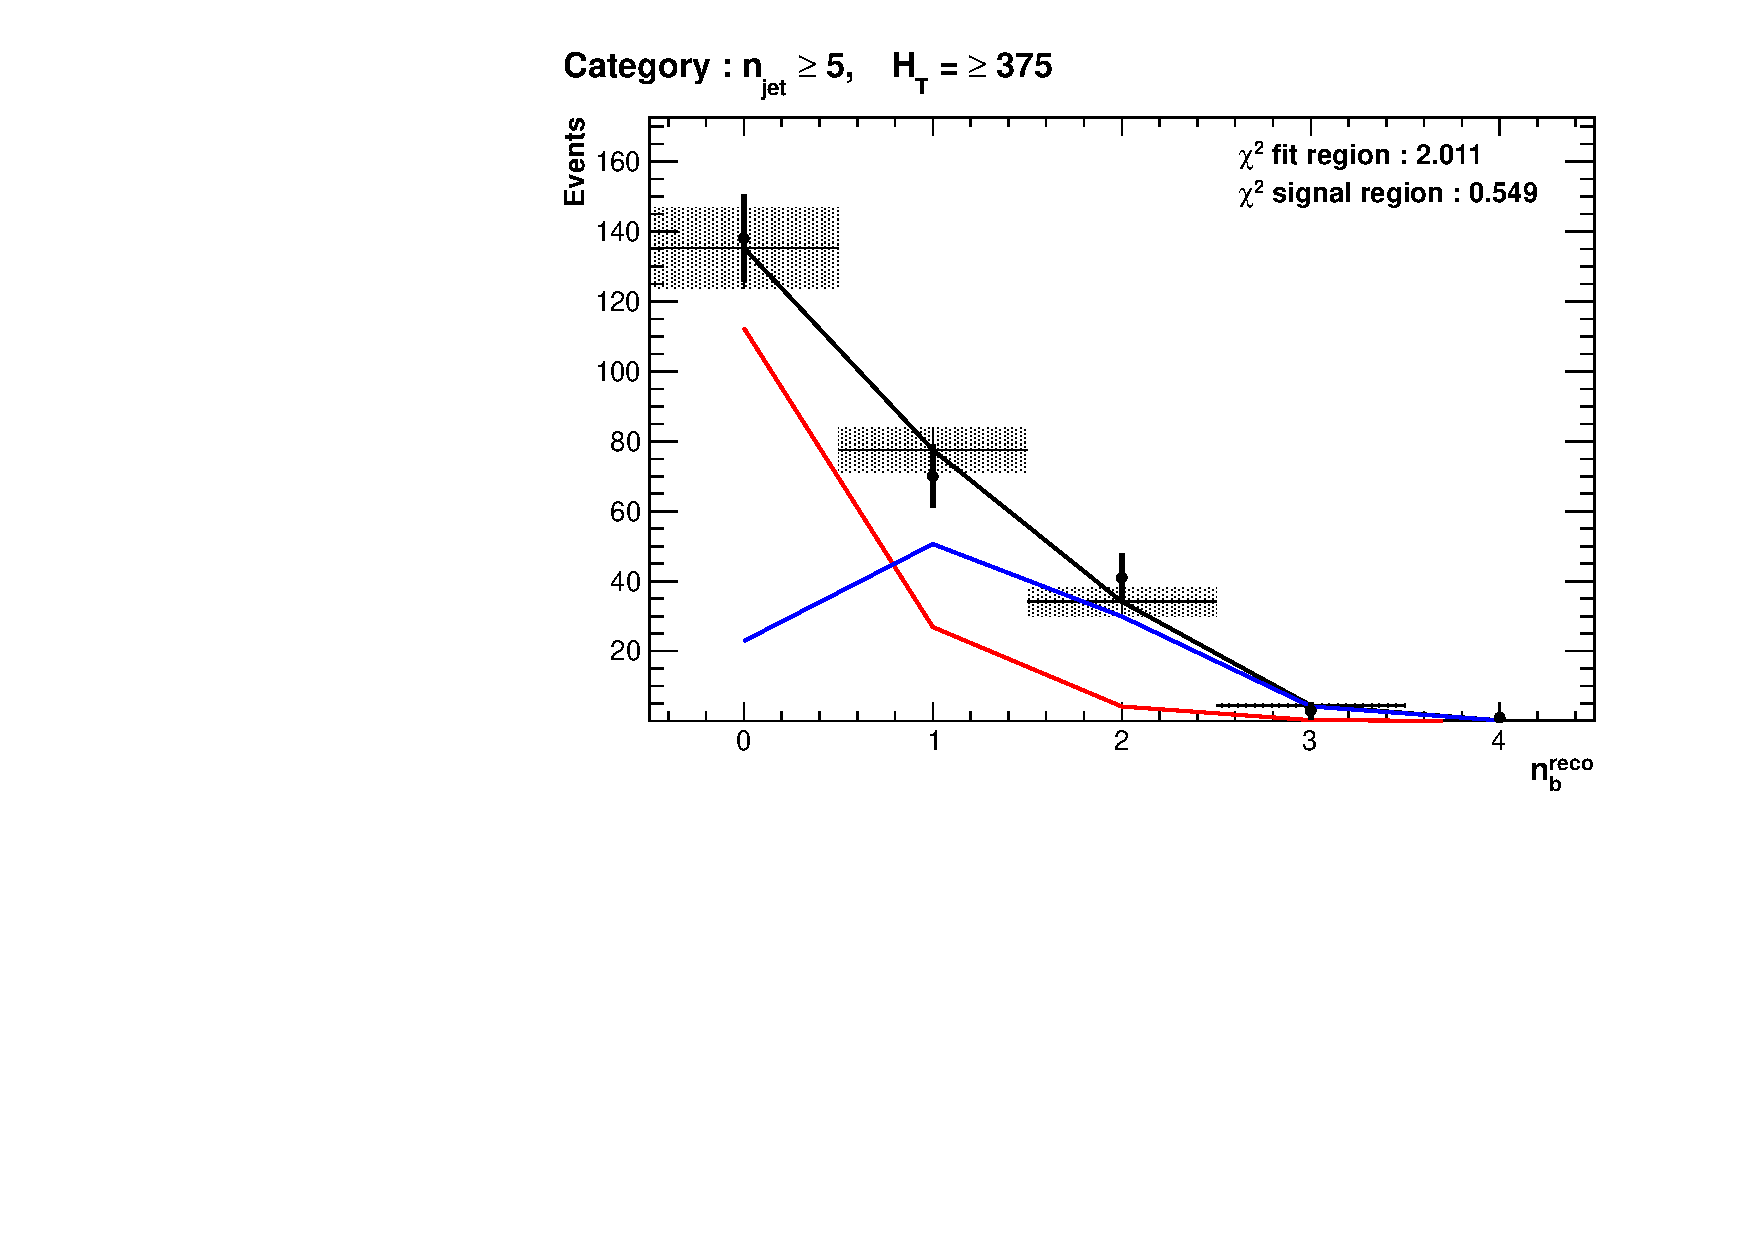
\includegraphics[width = 1.0\linewidth]{plots/TemplatesSignal/Final_Fit_To_Data_Normal_Medium_HTBin_Template_375_jet_mult_5.pdf}
\centering (b) Medium working point : $n_{jet} \geq$ 5 , \theht $>$ 375 
\end{minipage}
\begin{minipage}[b]{0.51\linewidth}
\centering
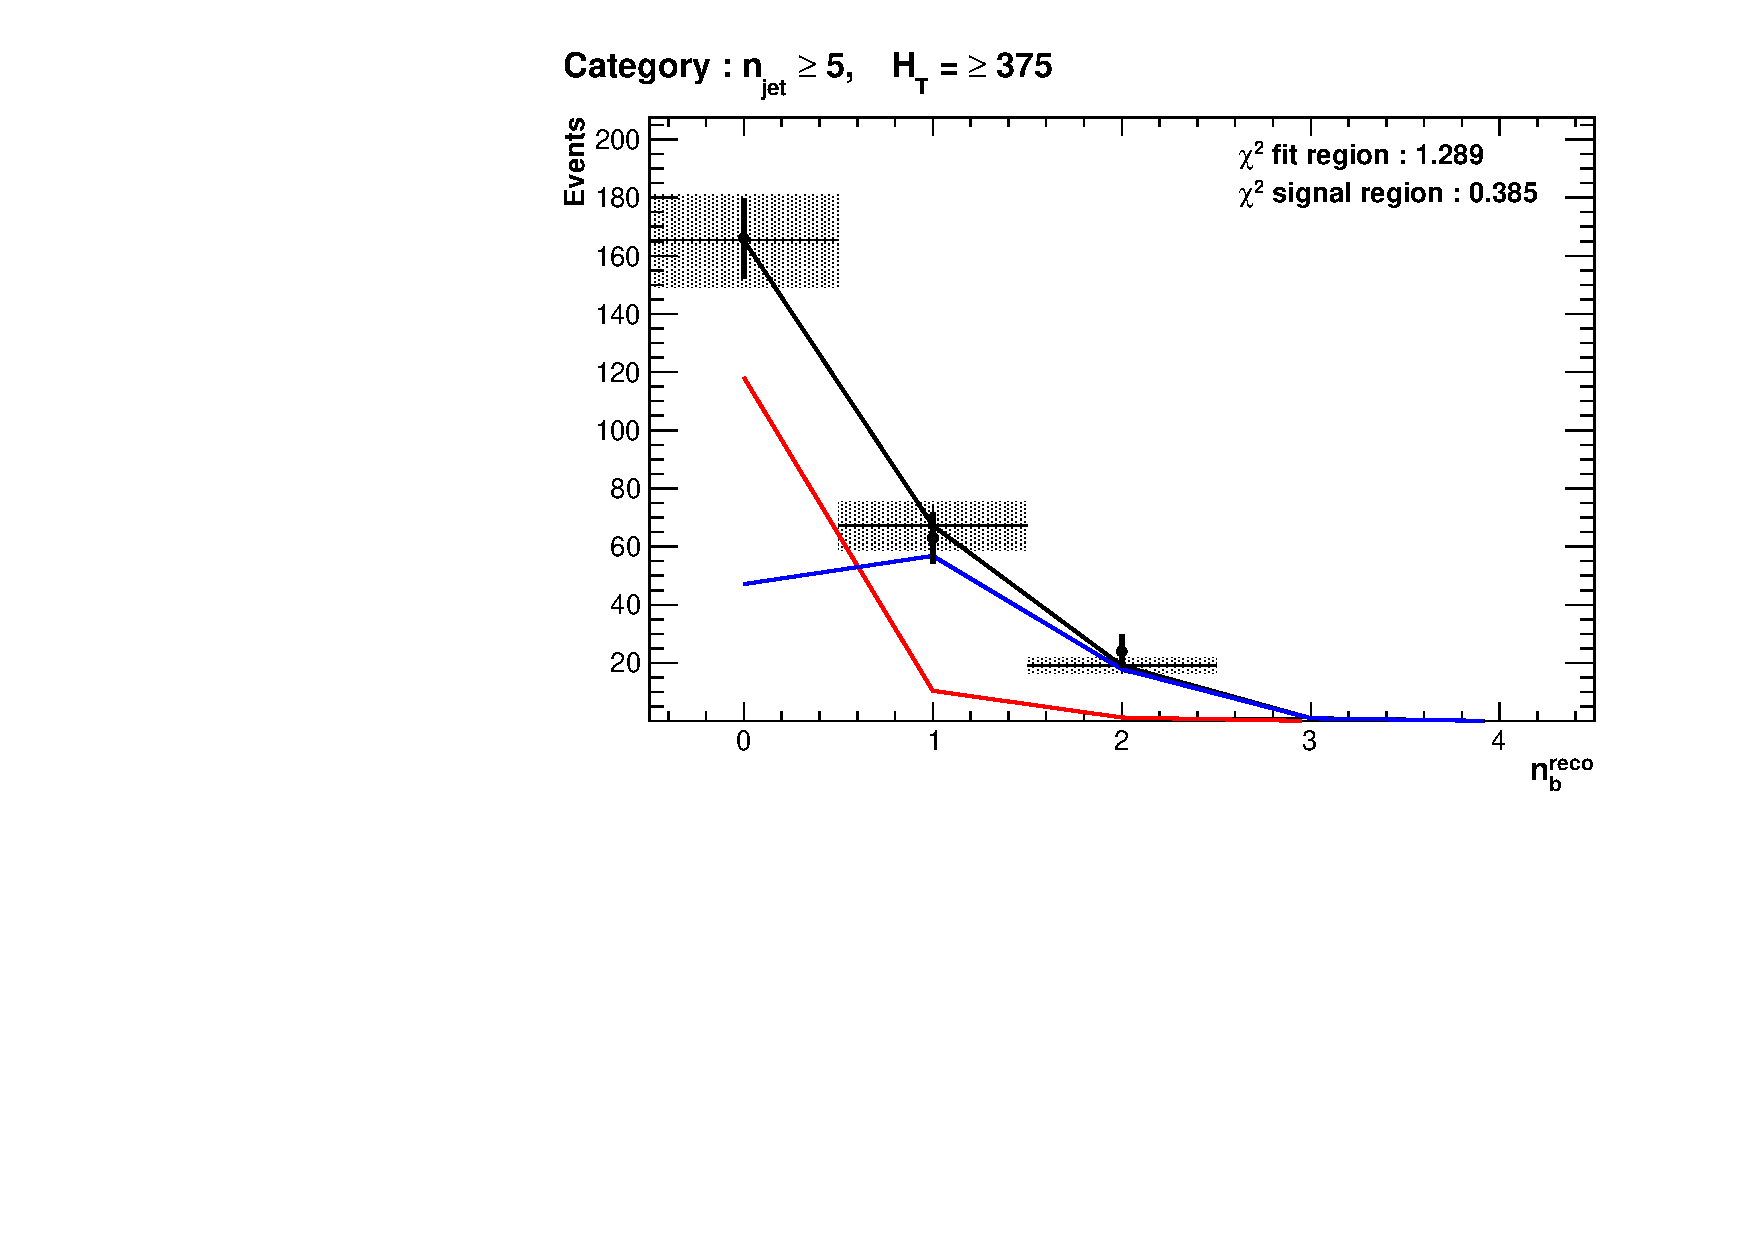
\includegraphics[width = 1.0\linewidth]{plots/TemplatesSignal/Final_Fit_To_Data_Normal_Tight_HTBin_Template_375_jet_mult_5.pdf}
\centering (c) Tight working point :  $n_{jet} \geq$ 5 , \theht $>$ 375 
\end{minipage}
\caption[Results of fitting the Z = 0 and Z = 2 templates in the $n_{b}^{reco}$ = 0-2 control region to data from the hadronic signal selection, in the $n_{jet} \geq 5$ and \theht $>$ 375 category for all \ac{CSV} working points.]{Results of fitting the Z = 0 and Z = 2 templates in the $n_{b}^{reco}$ = 0-2 control region to data from the hadronic signal selection, in the $n_{jet} \geq 5$ and \theht $>$ 375 category for all \ac{CSV} working points. Data is represented by the black circles with the blue, red and black lines representing the Z=0, Z=2 and combination of both templates respectively. Grey bands represent the uncertainty of the fit. The $\chi^{2}$ parameters represent the goodness of fit to the control and signal region.}
\label{fig:template_data_signal_njet5}
\end{figure}
\FloatBarrier

\begin{table}[h!]
\begin{center}
\footnotesize
\begin{tabular*}{0.95\textwidth}{@{\extracolsep{\fill}}lllll}
\cline{1-5}
\multicolumn{2}{c}{\theht} & 275-325 & 325-375 & $>$375 \\
\multicolumn{5}{c}{Loose working point} \\
\hline\hline
Data & \multirow{2}{*}{$n_{b} = 3$} & 198 & 85 & 126\\
Template &  & $207.1 \pm 28.7$ & $103.4 \pm 12.2$ & $124.98 \pm 14.4$ \\
Data & \multirow{2}{*}{$n_{b} = 4$} & 15 & 9 & 16 \\
Template &  & $15.9 \pm 5.4$ & $8.05 \pm 2.1$ & $13.1 \pm 3.2$ \\
\hline
\multicolumn{5}{c}{Medium working point} \\
\hline\hline
Data & \multirow{3}{*}{$n_{b} = 3$} & 33 & 16 & 14 \\
Template & & $25.4 \pm 4.0$ & $12.7 \pm 2.2$ & $19.9 \pm 2.9$ \\
\alphat ML Fit &  & $33.9 ^{+5.7}_{-4.3}$ & $16.3 ^{+1.9}_{-2.0}$ & $17.5 ^{+1.4}_{-1.4}$ \\ [1.1ex]
Data & \multirow{3}{*}{$n_{b} = 4$} & 1 & 0 & 2 \\
Template &  & $0.3 \pm 0.2$ & $0.3 \pm 0.1$ & $0.5 \pm 0.2$ \\
\alphat ML Fit &  & $0.9 ^{+0.4}_{-0.7}$ & $0.3 ^{+0.2}_{-0.2}$ & $0.6 ^{+0.3}_{-0.3}$ \\  [1.1ex]
\hline
\multicolumn{5}{c}{Tight working point} \\
\hline\hline
Data & \multirow{2}{*}{$n_{b} = 3$} & 5 & 2 & 0 \\
Template & & $4.03 \pm 0.8$ & $2.4 \pm 0.5$ & $3.1 \pm 0.6$ \\
Data & \multirow{2}{*}{$n_{b} = 4$} & 1 & 0 & 0 \\
Template & & $0.1 \pm 0.1$ & $0.1 \pm 0.1$ & $0.0 \pm 0.1$ \\
\end{tabular*}
\end{center}
\caption[Summary of the fit predictions in the $n_{b}^{reco}$ signal region of the \alphat hadronic signal selection, after combination of the $n_{jet} = 3, = 4, \geq 5$ categories. The predictions are extrapolated from a $n_{b}^{reco}$ = 0, 1, 2 control region using 11.7 fb$^{-1}$ of $\sqrt{s} = 8$\TeV data.]{Summary of the fit predictions in the $n_{b}^{reco}$ signal region of the \alphat hadronic signal selection, after combination of the $n_{jet} = 3, = 4, \geq 5$ categories. The predictions are extrapolated from a $n_{b}^{reco}$ = 0, 1, 2 control region using 11.7 fb$^{-1}$ of $\sqrt{s} = 8$\TeV data. The uncertainties quoted on the template yields are a combination of statistical and systematic uncertainties.}\label{tab:template_signal_table}
\end{table}

The numerical results and extrapolation to the $n_{b}^{reco} =$3, =4 bins for all \theht and working points are shown in Table \ref{tab:template_signal_table}. Included within the table are the combined \ac{SM} background predictions as determined by the maximum likelihood fit for both jet multiplicity categories of the \alphat analysis using the \ac{CSVM} tagger. No notable discrepancy is found in any of the three \ac{CSV} working points between the data and the background
expectations as determined by this method. The template predictions within the hadronic signal region are additionally found to be statistically compatible with the background predictions determined by the \alphat maximum likelihood fit which was first shown in Table \ref{tab:fitsdata}.

\section{Summary}
\label{subsec:templateconclusions}

A \ac{SUSY} signature such as one from gluino-induced third-generation squark production, would result in a final state with an underlying b-quark content greater than two. In order to be able to discriminate such signatures from the \ac{SM} background, templates are generated based on a parameterisation of \ac{SM} processes, where the underlying b-quarks per event is typically zero or two. These templates are then fit to data in a low $n_{b}^{reco}$ (0-2) control region in order to
extrapolate a prediction within a high $n_{b}^{reco}$ (3-4) signal region. This approach is built upon the assumptions that the defined control region is almost entirely free of any possible signal contamination from possible signal topologies with a small number of b-quarks in the final state.

The method was demonstrated both in simulation and also in data, using the \ac{SM} enriched \mupjets selection from the \alphat search. This was conducted to prove conceptually and experimentally that the method is valid and that there is adequate control over the measurement of the efficiency of each jet flavour for all working points of the \ac{CSV} tagger. Additionally this method was further applied to the hadronic signal region of the \alphat analysis, where good agreement is observed between the \ac{SM} background predictions from the template method, observations in data and also the background estimation procedure of the \alphat analysis.

